\documentclass[journal=jctcce]{achemso}

\usepackage[version=3]{mhchem}
\usepackage[T1]{fontenc}
\newcommand*\mycommand[1]{\texttt{\emph{#1}}}
\newcommand{\todo}[1]{\textcolor{red}{#1}}

\usepackage{rotating}
\usepackage{upgreek}				
\usepackage{xcolor}
\usepackage{booktabs}
\usepackage{multirow}
\usepackage{lmodern}
\usepackage{microtype}
\usepackage{xr}
\externaldocument{manuscriptPS}
\usepackage{soul} % for highlights with \hl{} 

\author{Hanne Antila}
\affiliation{Department of Theory and Bio-Systems, Max Planck Institute of Colloids and Interfaces, 14424 Potsdam, Germany}
\author{Pavel Buslaev}
\affiliation{Moscow Institute of Physics and Technology, Dolgoprudny, Russia}
\author{Fernando Favela-Rosales}
\affiliation{Departamento de Investigaci\'{o}n, Tecnol\'{o}gico Nacional de M\'{e}xico, Campus Zacatecas Occidente, M\'{e}xico}
\author{Tiago M. Ferreira}
\affiliation{Halle, Germany}
\author{Ivan Gushchin}
\affiliation{Moscow Institute of Physics and Technology, Dolgoprudny, Russia}
\author{Matti Javanainen}
\affiliation{Institute of Organic Chemistry and Biochemistry of the 
Czech Academy of Sciences, Flemingovo n\'{a}m. 542/2, CZ-16610 Prague 6, Czech Republic}
\author{Batuhan Kav}
\affiliation{Department of Theory and Bio-Systems, Max Planck Institute of Colloids and Interfaces, 14424 Potsdam, Germany}
\author{Jesper J. Madsen}
\affiliation{Department of Chemistry, The University of Chicago, Chicago, Illinois, United States of America}
\affiliation{Department of Global Health, College of Public Health, University of South Florida, Tampa, Florida, United States of America}
\author{Josef Melcr}
\affiliation{Institute of Organic Chemistry and Biochemistry of the 
Czech Academy of Sciences, Flemingovo n\'{a}m. 542/2, CZ-16610 Prague 6, Czech Republic}
\author{Markus Miettinen}
\affiliation{Department of Theory and Bio-Systems, Max Planck Institute of Colloids and Interfaces, 14424 Potsdam, Germany}
\author{Ricky Nencini}
\affiliation{Institute of Organic Chemistry and Biochemistry of the 
Czech Academy of Sciences, Flemingovo n\'{a}m. 542/2, CZ-16610 Prague 6, Czech Republic}
\author{O. H. Samuli Ollila}
\email{samuli.ollila@helsinki.fi}
%\homepage[]{Your web page}
\affiliation{Institute of Organic Chemistry and Biochemistry of the 
Czech Academy of Sciences, Flemingovo n\'{a}m. 542/2, CZ-16610 Prague 6, Czech Republic}
\affiliation{Institute of Biotechnology, University of Helsinki}
\author{Thomas J. Piggot}
\affiliation{Chemistry, University of Southampton, Highfield, Southampton SO17 1BJ, U.K}


\SectionNumbersOn

\renewcommand{\thetable}{S\arabic{table}}%
\renewcommand{\thefigure}{S\arabic{figure}}%
\renewcommand{\thesection}{S\arabic{section}}%
\renewcommand{\thepage}{S\arabic{page}}%

\title{ Supporting Information:\\ Headgroup structure and cation binding in phosphatidylserine lipid bilayers}

\begin{document}

%\newpage
%\tableofcontents

\section{Simulated systems}


%\begin{table*}[!p]
\begin{sidewaystable*}[!p]
\centering
\caption{The list of POPC:POPS mixtures simulated with different amounts of added monovalent ions. 
  The salt concentrations are calculated as [salt]=N$_{\rm c} \times$[water]\,/\,N$_{\rm w}$, where [water]\,=\,55.5~M.
  This corresponds the concentration in buffer before solvating lipids, which are
  reported in the experiments by Roux et al.~\cite{roux90}.
  % The simulation details are given in the supplementary information.
  % The lipid force fields named as in our previous work~\cite{botan15}.
}\label{mixedIONsystemsMONOVALENT}
%begin{minipage}[t]{\textwidth}
\begin{tabular}{l c c c c c c c c c}
  lipid/counter-ions & force field for lipids / ions & \footnote{Excess Na$^+$ or K$^+$ concentration}C$_{\rm ci}$ (M) &  \footnote{Number of lipid molecules with largest mole fraction}N$_{\rm l}$   &  \footnote{Number of water molecules}N$_{\rm w}$   & \footnote{Number of additional cations}N$_{\rm c}$  & \footnote{Simulation temperature}T (K)  & \footnote{Total simulation time}t$_{{\rm sim}}$(ns) & \footnote{Time used for analyses}t$_{{\rm anal}}$ (ns) &   \footnote{Reference for simulation files}files\\
  \hline
%    POPC:POPS (5:1)/K$^+$  & CHARMM36 \cite{klauda10,venable13} &0 & 0  & 110:22 & 4935 & 0  & 298  & 100 & 100 \todoi{Equilibration?} & \cite{charmm36pops+83popcT298K}  \\
    POPC:POPS (5:1)/K$^+$  & CHARMM36 \cite{klauda10,venable13} &0 & 250:50 & 11207 & 0  & 298  & 200 & 180   & \citenum{POPC5POPS1noCaClCHARMM}  \\
    POPC:POPS (5:1)/K$^+$  & CHARMM36 \cite{klauda10,venable13} &0     & 110:22 & 4620  & 0  & 298  & 500 & 100 & \citenum{charmm36pops+83popcT298Kpiggot}  \\
    POPC:POPS (5:1)/K$^+$  & CHARMM36 \cite{klauda10,venable13} &0.45  & 110:22 & 4926  & 40 & 298  & 200 & 150 & \citenum{charmm36pops+83popcT298Kwith450mMK}  \\
    POPC:POPS (5:1)/K$^+$  & CHARMM36 \cite{klauda10,venable13} &0.89  & 110:22 & 4946  & 79 & 298  & 200 & 150 & \citenum{charmm36pops+83popcT298Kwith890mMK}  \\
    POPC:POPS (5:1)/Na$^+$ & CHARMM36 \cite{klauda10,venable13} &0     & 110:22 & 4620  & 0  & 298  & 500 & 100 & \citenum{charmm36pops+83popcT298KpiggotSODIUM}  \\
    POPC:POPS (5:1)/Na$^+$  & CHARMM36 \cite{klauda10,venable13} &0.44 & 110:22 & 4965  & 39 & 298  & 200 & 150 & \citenum{charmm36pops+83popcT298Kwith440mMNa}  \\
    POPC:POPS (5:1)/Na$^+$  & CHARMM36 \cite{klauda10,venable13} &0.89 & 110:22 & 4932  & 79 & 298  & 200 & 150 & \citenum{charmm36pops+83popcT298Kwith890mMNa}  \\
    \hline
    POPC:POPS (5:1)/K$^+$  & MacRog \cite{maciejewski14} &0    & 120:24 & 5760 & 0    & 298  & 400 & 250 & \citenum{POPCpopsMACROG}  \\
    POPC:POPS (5:1)/K$^+$  & MacRog \cite{maciejewski14} &0.50 & 120:24 & 5760 & 52   & 298  & 300 & 200 & \citenum{POPCpopsMACROGwithK}  \\
    POPC:POPS (5:1)/K$^+$  & MacRog \cite{maciejewski14} &1.00 & 120:24 & 5760 & 104  & 298  & 300 & 200 & \citenum{POPCpopsMACROGwithK}  \\
    POPC:POPS (5:1)/K$^+$  & MacRog \cite{maciejewski14} &2.00 & 120:24 & 5760 & 208  & 298  & 300 & 200 & \citenum{POPCpopsMACROGwithK}  \\
    POPC:POPS (5:1)/K$^+$  & MacRog \cite{maciejewski14} &3.00 & 120:24 & 5760 & 311  & 298  & 300 & 200 & \citenum{POPCpopsMACROGwithK}  \\
    \hline
    POPC:POPS (5:1)/K$^+$  & Lipid14/17 \cite{dickson14,gould18} &0     & 120:24 & 5760 & 0   & 298  & 500 & 200 & \citenum{POPCpopsLIPID17withKCI}  \\
    POPC:POPS (5:1)/K$^+$  & Lipid14/17 \cite{dickson14,gould18} &0.50  & 120:24 & 5760 & 54   & 298  & 300 & 200 & \citenum{POPCpopsLIPID17withK}  \\
    POPC:POPS (5:1)/K$^+$  & Lipid14/17 \cite{dickson14,gould18} &1.00  & 120:24 & 5760 & 104  & 298  & 300 & 200 & \citenum{POPCpopsLIPID17withK}  \\
    POPC:POPS (5:1)/K$^+$  & Lipid14/17 \cite{dickson14,gould18} &2.00  & 120:24 & 5760 & 208  & 298  & 300 & 200 & \citenum{POPCpopsLIPID17withK}  \\
    POPC:POPS (5:1)/K$^+$  & Lipid14/17 \cite{dickson14,gould18} &3.00  & 120:24 & 5760 & 311  & 298  & 300 & 200 & \citenum{POPCpopsLIPID17withK}  \\
    POPC:POPS (5:1)/K$^+$  & Lipid14/17 \cite{dickson14,gould18} &4.00  & 120:24 & 5760 & 415  & 298  & 300 & 200 & \citenum{POPCpopsLIPID17withK}  \\
    POPC:POPS (5:1)/Na$^+$  & Lipid14/17 \cite{dickson14,gould18} &0    & 120:24 & 5760 & 0   & 298  & 500 & 200 & \citenum{POPCpopsLIPID17withNaCI}  \\
    POPC:POPS (5:1)/Na$^+$  & Lipid14/17 \cite{dickson14,gould18} &0.50 & 120:24 & 5760 & 54   & 298  & 300 & 200 & \citenum{POPCpopsLIPID17withNa}  \\
    POPC:POPS (5:1)/Na$^+$  & Lipid14/17 \cite{dickson14,gould18} &1.00 & 120:24 & 5760 & 104   & 298  & 300 & 200 & \citenum{POPCpopsLIPID17withNa}  \\
    POPC:POPS (5:1)/Na$^+$  & Lipid14/17 \cite{dickson14,gould18} &2.00 & 120:24 & 5760 & 208   & 298  & 300 & 200 & \citenum{POPCpopsLIPID17withNa}  \\
    POPC:POPS (5:1)/Na$^+$  & Lipid14/17 \cite{dickson14,gould18} &3.00 & 120:24 & 5760 & 311   & 298  & 300 & 200 & \citenum{POPCpopsLIPID17withNa}  \\
    POPC:POPS (5:1)/Na$^+$  & Lipid14/17 \cite{dickson14,gould18} &4.00 & 120:24 & 5760 & 415   & 298  & 300 & 200 & \citenum{POPCpopsLIPID17withNa}  \\
    \hline
    POPC:POPS (4:1)/Na$^+$  & Berger \cite{tieleman99,mukhopadhyay04} &0    & 102:26 & 4290 & 0   & 310  & 120 & 80 & \citenum{bergerPOPSPOPC4:1mixtureT310K}  \\
    POPC:POPS (4:1)/Na$^+$  & Berger \cite{tieleman99,mukhopadhyay04} &1.03 & 102:26 & 4290 & 80  & 310  & 200 & 50 & \citenum{POPCpopsBERGERwith1000mMNa}  \\
\end{tabular}
%\end{minipage}
\end{sidewaystable*} 

% \end{table*}




\subsection{CHARMM36}

\noindent
    {\it POPC bilayer.} Previously published values \cite{botan15} calculated from the data
    available from Ref. \citenum{charmmPOPC512files} are used.
% It should be noted that pure POPC are ran with Gromacs 4, but the results with
% PS are ran with Gromacs 5. This has significant effect on acyl chains:
% https://github.com/NMRLipids/NmrLipidsCholXray/issues/4
% but the effect to headgroups is small
% https://github.com/NMRLipids/MATCH/blob/master/Data/Lipid_Bilayers/POPC/T303K/MODEL_CHARMM36_GROMACS4.5/Headgroup_Glycerol_Order_Parameters_Simulation.dat
% https://github.com/NMRLipids/MATCH/blob/master/Data/Lipid_Bilayers/POPC/T303K/MODEL_CHARMM36_GROMACS5.1.2/Headgroup_Glycerol_Order_Parameters_Simulation.dat}

\noindent
{\it DOPS and POPS bilayers.}
%The data in Table \ref{PSsystems} and Refs \citenum{charmm36DOPS303K,charmm36POPS298K,charmm36POPS298Kpotassium}
Starting structures for CHARMM36 DOPS and POPS simulations were constructed using the CHARMM-GUI webserver~\cite{lee16,jo18}.
The systems contained a total of 128 lipids (64 per leaflet of the membrane), 35 waters per lipid, and 128 Na$^+$ ions.
Force field parameters for DOPS and POPS were taken from Venable et al. and included the modified parameters for interactions
with Na$^+$ ions \cite{venable13}. Water was treated using the CHARMM TIP3P model \cite{durell94,eyal96}.
%https://pubs.acs.org/doi/10.1021/j100059a038 and https://aip.scitation.org/doi/10.1063/1.472061].
For POPS, an identical system was also constructed in which the 128 Na$^+$ ions were replaced with 128 K$^+$ ions.

Simulations of these systems were performed for 500~ns using GROMACS, version 5.0.6 \cite{abraham2015gromacs}.
A 2~fs timestep was applied during the simulations, and the LINCS algorithm was used to constrain all bonds to hydrogen atoms \cite{hess97,hess07}.
For each of the DOPS and POPS systems, two simulations were performed using different randomly assigned starting velocities.
The simulations were maintained at temperatures of 303~K and 298~K for DOPS and POPS respectively using the Nos\'{e}--Hoover thermostat \cite{nose84,hoover85}
with a coupling constant of 1~ps. A pressure of 1~bar was maintained using the Parrinello--Rahman \cite{parrinello81} method with a coupling constant of 5~ps.
Pressure coupling was applied in a semi-isotropic manner with the $x$ and $y$ dimensions, in the plane of the bilayer, fluctuating independently of the $z$ dimension.
Standard CHARMM36 force field methods were applied for the simulation cut-offs: van der Waals interactions were truncated at 1.2~nm with the interactions
switched off between 1.0~nm and 1.2~nm; Coulombic interactions were truncated at 1.2~nm with long-range interactions treated using PME~\cite{darden93,essman95}.

Analyses on these simulations was performed on the final 100~ns of the simulations.



\noindent
{\it POPC:POPS mixtures without additional ions}
Simulations of POPC:POPS (5:1) mixtures containing a total of 132 lipids (110 POPC and 22 POPS) were constructed using the CHARMM-GUI~\cite{lee16,jo18}.
Two identical systems were constructed, apart from one system was neutralised through the addition of 22 Na$^+$ ions while the other system
contained 22 K$^+$ ions. As per the pure POPS CHARMM36 simulations, 35 water per lipid were added. All other system and simulation parameters
and settings were identical to those used in the CHARMM36 POPS simulations.


%Simulations of POPC:POPS (5:1) mixture containing total 132 (110:22) lipids
%with potassium and sodium countertions were ran using CHARMM36 force field.
%The data are available from Refs. \citenum{charmm36pops+83popcT298Kpiggot}
%and \citenum{charmm36pops+83popcT298KpiggotSODIUM}, respectively\todo{T. Piggot, please write simulation details}.

Simulations of POPC:POPS (5:1) ans POPC:POPS (1:1) mixtures containing total 300 lipids (250:50 and 150:150, respectively)
with neutralizing potassium countertions 
%ran using CHARMM36 force field.
%The data are available from Refs. \citenum{POPC5POPS1noCaClCHARMM} and \citenum{POPC1POPS1noCaClCHARMM}.
%POPC:POPS (both 1:1 and 5:1) mixtures
were prepared
%with 300 lipids in total
%with the  ions
using the CHARMM-GUI \cite{lee16,jo18}. The systems were simulated using Gromacs 5 \cite{abraham2015gromacs}
and CHARMM36 force field with the simulation parameters given by the CHARMM-GUI at 298~K. For further details see table \ref{mixedIONsystemsMONOVALENT}. 
 \\

\noindent
{\it POPC:POPS (5:1) mixtures with additional monovalent ions.}
POPC:POPS (110:22) mixtures containing total 132 lipids with the additional
potassium or sodium ions corresponding concentrations of $\sim$450~mM and 890~mM
were generated with the CHARMM-GUI \cite{lee16,jo18}. Systems were simulated using
Gromacs 5 \cite{abraham2015gromacs} and CHARMM36 force field with the simulation
parameters given by the CHARMM-GUI at 298~K. For further details, simulation files
and data, see table \ref{mixedIONsystemsMONOVALENT} and
Refs. \citenum{charmm36pops+83popcT298Kwith450mMK,charmm36pops+83popcT298Kwith890mMK,charmm36pops+83popcT298Kwith440mMNa,charmm36pops+83popcT298Kwith890mMNa}. \\


\noindent
{\it POPC:POPS (5:1) mixtures with additional calcium} 
POPC:POPS (5:1) mixtures containing total 300 (250:50) lipids
%were simulated with the additional calcium concentrations.
%The data is available from Refs. \citenum{POPC5POPS1withCaClCHARMM} and \citenum{POPC5POPS1with1MCaClCHARMM}.
and 0.26~M and 1~M CaCl$_2$ were prepared using the CHARMM-GUI \cite{lee16,jo18}.
Systems were simulated using Gromacs 5 \cite{abraham2015gromacs} and CHARMM36 force field with the simulation parameters given
by the CHARMM-GUI at 298~K.

\subsection{CHARMM36ua}
\noindent
{\it DOPS and POPS bilayers.} 
%The data in Table \ref{PSsystems} and Refs \citenum{charmm36uaDOPS303K,charmm36uaPOPS298K}
Starting structures for CHARMM36-UA DOPS and POPS simulations were taken from those generated for the CHARMM36 simulations (see above),
with any extraneous hydrogen atoms removed in the lipid tails. Force field parameters for DOPS and POPS were constructed through a
combination of the published CHARMM36 PS~\cite{venable13} and CHARMM36-UA PC parameters~\cite{lee14}.
% [REF: https://pubs.acs.org/doi/10.1021/jp410344g].
All other simulation parameters and conditions were identical to those described for the CHARMM36 all-atom DOPS and POPS simulations.


\subsection{MacRog}
\noindent
{\it POPC bilayers.} 
% \todo{For example this data set has pretty good description of simulation details in the
% reference. I am not sure how much we should repeat these in here.}
The POPC bilayer consisting of a total of 128 lipids was constructed from single lipid structure taken 
from Ref.~\citenum{kulig15c}. The bilayer was hydrated by a total of 5120 water 
molecules, corresponding to 40 water molecules per lipid.
The MacRog lipid parameters \cite{kulig15b}, obtained from Ref.~\citenum{kulig15c}, were used,
along with the TIP3P water model~\cite{jorgensen83}. The simulation parameters were identical to those used for 
POPC/POPC mixtures with the MacRog force field, see below. The simulation was run for 200~ns using Gromacs 2016.3~\cite{abraham2015gromacs}, 
out of which 150~ns were used for analyses. The simulation data and related files are available from Ref. \citenum{macrogPOPC298K}.

\noindent
{\it POPS bilayers with Na$^+$ counterions.}
%The data in Table \ref{PSsystems} and Refs \citenum{macrogPOPS298Kcorrect,macrogPOPS298KwithK}
%\todo{T. Piggot and M. Javanainen, please write simulation details} \\
%\hl{Piggot: please write about system with Na$^+$ counterions}.
Force field parameters for POPS simulations with the MacRog OPLS-AA force field~\cite{maciejewski14,kulig15b,rog16}
were constructed manually using the provided PS parameters as a guide~\cite{rog16}. The original parameters were
not used due to an incorrect arrangement of the {\it sn}-1 and {\it sn}-2 tails (i.e. the lipid was OPPS and not POPS).
The corrected parameters are available from Ref.~\citenum{macrogPOPS298KwithK}.
The starting structure was the same as that used in the CHARMM36 POPS simulations (with Na$^+$ ions) and was converted into
the correct format using a script to adjust the atom order. Water was treated using the TIP3P model~\cite{jorgensen83}.
Simulation parameters were chosen to closely mimic those used in the original force field publications~\cite{maciejewski14,kulig15b,rog16}:
van der Waals interactions were truncated at 1.0~nm with a dispersion correction applied to the energy and pressure;
Long-range Coulombic interactions were treated with PME beyond a system-optimized cut-off.
All other simulation settings were identical to those described above for the CHARMM36 DOPS and POPS simulations,
including use of the Verlet cut-off scheme~\cite{Pall13}, apart from the use of LINCS to constrain all bonds during these simulations.
Simulations with the group cut-off scheme gave slightly lower area per molecule ($\sim$~50\AA$^2$) than
the simulations with Verlet cut-off ($\sim$~52\AA$^2$).

\noindent
{\it POPS bilayers with K$^+$ counterions.}
The membrane with sodium counterions was further simulated after replacing Na$^+$ counterions by K$^+$ ones, which 
were described by the \AA{}qvist parameters \cite{aqvist90}. Other topologies
were unchanged. The simulation parameters were the same as used for the POPC/POPS mixtures with 
the MacRog force field, see below. The simulation was run for 200~ns, out of which 150~ns was used 
in the analyses.

\noindent
{\it POPC:POPS (5:1) mixtures with additional potassium ions} \\
%The data in Table \ref{mixedIONsystems} and Refs \citenum{POPCpopsMACROG,POPCpopsMACROGwithK}
The bilayers containing a total of 120 POPC and 24 POPS molecules distributed evenly among the 
two leaflets were set up using CHARMM-GUI \cite{lee16,jo18}.
The bilayers were solvated by 5760 water molecules, corresponding to 40 water molecules for lipid.
Additionally, 24 potassium ions were added to neutralize the charge of the POPS head groups.
These bilayers were simulated using Gromacs 2016.3~\cite{abraham2015gromacs} in the presence of counterions only, as well as together with different
concentrations of CaCl$_2$ or KCl. For the former, concentrations of 100~mM, 300~mM, 1~M, and 3~M 
were considered, which corresponded to the amounts of 10/20, 31/62, 104/208, and 311/622 
of Ca$^{2+}$/Cl$^-$ ions. For membranes with KCl, concentrations of 500~mM, 1~M, 2~M, and 3~M of 
were considered, corresponding to 52, 104, 208, or 311 pairs of K$^+$ and Cl$^-$ ions.

The lipids were described using the MacRog model \cite{maciejewski14,kulig15b,rog16}. The POPC topologies were obtained from 
Ref.~\citenum{kulig15c}, whereas the POPS topology was adapted from OPPS topology in
Ref.~\citenum{rog16} by reversing the order of acyl chains.
The initial structures from CHARMM-GUI were used because they have the
naturally occurring L stereoisomer in the POPS head group, instead of the 
the D stereoisomer present in Ref.~\citenum{rog16}.
TIP3P model \cite{jorgensen83} was used for water, and the \AA{}qvist parameters 
\cite{aqvist90}, standard for the OPLS force field, were employed for the ions. 

The simulation parameters were taken from Ref.~\citenum{rog16}. 
Periodic boundary conditions were employed in all dimensions. The list of neighbors was updated every step. 
%\hl{I used nstlist=1 because it's used in the mdp in the article quoted. In DOI: 10.1021/jp5016627, nstlist=10 is used}
The Lennard-Jones interactions were cut off at 1~nm, whereas the smooth particle mesh Ewald algorithm 
\cite{essman95} was used for long-range electrostatics. Dispersion correction \cite{shirts07} 
was applied to both energy and pressure. Temperature was kept constant at 298~K using the 
Nos\'{e}--Hoover thermostat \cite{nose84,hoover85}. The lipids and 
the solvent were coupled separately, and a time constant of 0.4~ps was employed. Pressure was 
maintained semi-isotropically at 1~bar using the Parrinello--Rahman barostat with a time constant of 1~ps 
\cite{parrinello81}. All non-water bonds were constrained with the LINCS algorithm 
\cite{hess97,hess07},
whereas the bonds in water molecules were constrained using SETTLE \cite{miyamoto92}.
The integration time step was set to 2~fs, and the simulations were performed either for 400~ns 
(only counterions), 300~ns (systems with KCl), or 600~ns (systems with CaCl$_2$). The last 
250, 200, or 300~ns of the simulations were included in the analyses, respectively.

\subsection{Lipid17}
{\it DOPS and POPS bilayers.} 
The structure of the bilayers with 128 DOPS or 128 POPS lipids were
obtained from CHARMM-GUI~\cite{lee16,jo18}. Bilayers are solvated with
4480 water molecules resulting in 31.1 water molecules per lipid. For
each system, 128 NaCl molecules are added to neutralize the system.
In all simulations, TIP3P~\cite{jorgensen1983comparison} was used as the solvent. SETTLE~\cite{miyamoto92} algorithm was employed 
to constrain the bonds in TIP3P water molecules. Simulations were ran using Amber18 simulation package \cite{amber18md}
and lipid parameters were obtained from Amber Lipid17 force field \cite{gould18}. For the ions, one set of simulations were run with Joung--Cheatham
ion parameters~\cite{joung2008determination} and one set of simulations were run with ff99SB (\AA{}qvist)~\cite{aqvist90} ion parameters.
The data in Table~\ref{PSsystems} and Refs~\citenum{lipid17POPSjcions,lipid17POPSff99ions,lipid17DOPSjcions,lipid17DOPSff99ions} contain
the number of molecules in simulations, related simulation files and trajectories.

Each bilayer structure was first minimized for 2500 steps with steepest
descent and an additional 2500 step with the conjugate gradient
algorithms while restraining the solvent and ion molecules with a force
constant 500~kcal~mol$^{-1}$~\AA{}$^{-2}$. An additional minimization
step was used with the same parameters after removing the constraints on
the solvent and ion molecules. During the minimization procedure,
non-periodic boundary conditions were applied, no pressure scaling was
used and none of the bonds were restrained. A three step heating
procedure was applied: in the first heating step the system temperature
is increased from 0.0~K to 100.0~K using Langevin thermostat with
5.0~ps$^{-1}$ collision frequency while restraining the lipid positions
with harmonic springs of force constant
20.0~kcal~mol$^{-1}$~\AA{}$^{-1}$ at constant volume without periodic
boundary conditions. In the second heating step, the system temperature
was increased from 100.0~K to 200.0~K using Langevin thermostat with
5.0~ps$^{-1}$ collision frequency within 10000 steps while restraining
the lipid positions with harmonic springs of force constant
10.0~kcal~mol$^{-1}$~\AA{}$^{-1}$ at constant volume. In the third
heating step, the system temperature is increased from 200.0~K to
303.0~K within 10000 steps using Langevin thermostat with 5.0~ps$^{-1}$
collision frequency while restraining the lipid positions with harmonic
springs of force constant 10.0~kcal~mol$^{-1}$~\AA{}$^{-1}$ at 1~bar
constant pressure using Berendsen barostat with 3.0~ps relaxation time.
From the second heating step onward, periodic boundary conditions in all
dimensions were applied. The semi-isotropic pressure coupling along
\textit{xy}-plane was employed and the surface tension was set to
0.0~dyn explicitely. After the third heating step, each structure is
equilibriated for 100~ns at 1~bar and 303~K constant pressure using
Berendsen barostat and temperature using Langevin thermostat,
respectively. For the equilibriation step, semi-isotropic pressure
coupling along \textit{xy}-plane was employed and the surface tension
was set to 0.0~dyn explicitely. For all heating and equilibration steps,
the lengths of the hydrogen containing bonds were restrained using SHAKE
algorithm and a time step of 2~fs was used. In all steps with periodic
boundary conditions, the non-bonded interactions are calculated with
particle mesh Ewald~\cite{essman95} using 1.0~nm cutoff.

For the production runs, the temperature and pressure were set to 303~K
and 1~bar, using Langevin thermostat with 1.0~ps$^{-1}$ collision
frequency and Berendsen barostat with 1.0~ps relaxation time,
respectively. Periodic boundary conditions were applied in all
dimensions and the non-bonded interactions are calculated with particle
mesh Ewald~\cite{essman95} using 1.0~nm cutoff. The lengths of the
hydrogen containing bonds were constrained using SHAKE algorithm and a
time step of 2~fs was used. Trajectories are saved in every 10~ps
intervals. Two independent trajectories of 500~ns long was generated and
the last 200~ns portions were used for the analysis.

\noindent
{\it POPC:POPS (5:1) mixtures with additional potassium and sodium ions} 
The initial structure of the bilayers with 120 POPC and 24 POPS lipids were obtained from CHARMM-GUI~\cite{lee16,jo18}.
Bilayers were solvated with 5760 TIP3P water molecules~\cite{jorgensen1983comparison}. For the simulations of the lipids and ions,
the Amber Lipid 17 \cite{gould18} and ff99SB~\cite{aqvist90} force fields were used, respectively.
Simulations were ran using Amber18 simulation package \cite{amber18md} 
The simulation steps are the same as the the simulations of
DOPS and POPS bilayers described above, with the only difference that the total simulation time was 300~ns, of which last 200~ns
was used for the analysis. The number of ions in each specific system is given in Table~\ref{mixedIONsystemsMONOVALENT}.
The trajectory files can be found in Refs~\citenum{POPCpopsLIPID17withKCI,POPCpopsLIPID17withK,POPCpopsLIPID17withNaCI,POPCpopsLIPID17withNa}.

\noindent
{\it POPC:POPS (5:1) mixtures with additional calcium chloride concentration with default Amber parameters} 
%The data in Table \ref{mixedIONsystems} and Refs \citenum{lipid17_cacl_series,POPCpopsLIPID17withCaCl} 
%We have performed two sets of simulations of POPC:POPS (5:1) mixtures using Amber Lipid17 force field \cite{gould18}
%with additional calcium chloride concentrations, 
%which employed different simulation engines and parameters for ions.
Simulations were performed using Amber18 simulation package \cite{amber18md} with ff99SB~\cite{aqvist90} ion parameters and Amber Lipid17~\cite{gould18} force field. 
Number of ions and water molecules for this set of simulations are shown in Table~\ref{mixedIONsystems}.
The simulation details, minimization, heating, and equilibration runs are the same as described above for the other POPC:POPS (5:1) simulations with Amber Lipid17 forcefield. 
For each ion concentration, 100~ns equilibration runs were followed by 300~ns production runs with two independent trajectories, of which last 200~ns were used for the analysis.
The trajectory files can be found from Ref~\citenum{POPCpopsLIPID17withCaCl}.

\noindent
{\it POPC:POPS (5:1) mixtures with additional calcium chloride concentration with Dang ion parameters} 
The Lipid17 parameters for POPS were obtained from AmberTools18 \cite{amber18md} 
and converted to Gromacs format using acpype \cite{silva12}.  
The previously generated \cite{botan15} Lipid14 parameters for POPC in Gromacs format were downloaded from Ref.~\citenum{lipid14files}. 
Dang parameters for ions \cite{smith94, dang06} were used.
% Another set of simulations with Lipid17 force field for lipids \cite{gould18}
Initial structures were generated using CHARMM-GUI~\cite{lee16,jo18} 
and simulations were performed using the GROMACS 2018 simulation package~\cite{abraham2015gromacs}
with the time step of 2~fs. 
The non-bonded interactions were calculated directly within 1.0~nm cutoff using the Verlet scheme \cite{Pall13}, 
and the long-range electrostatic forces were calculated using particle mesh Ewald~\cite{essman95}. 
The bond lengths of hydrogen atoms were constrained using LINCS algorithm \cite{hess97}.
Temperature was coupled to the velocity rescaling thermostat \cite{bussi07} at 298~K with a coupling constant of 1~ps.
Pressure was coupled to the Parrinello--Rahman barostat \cite{parrinello81} at 1~bar with a coupling constant of 10~ps. 
The compositions of individual simulations are shown in Table~\ref{mixedIONsystems}. 
The systems were equilibrated 50~ns prior to production simulations used for analysis,
which are available in Ref.~\citenum{lipid17_cacl_series} including the simulation settings. 
Topologies in a format for the GROMACS package are available in the repository \citenum{ECCpops}. 


\subsection{Slipids}
%
%\noindent
%{\it POPS}
%\todo{POPS \cite{slipidsPOPS298K} to be written by Piggot}%%
%
%\noindent
%{\it DOPS with 128 lipids.}
%\todo{DOPS with 128 lipids \cite{slipidsDOPS303K} to be written by Piggot}
%
\noindent
{\it POPS and DOPS with 128 lipids}
Starting structures for the Slipids POPS and DOPS (with 128 lipids) simulations were the same as constructed
for the CHARMM36 simulations. Force field parameters were taken from the published Slipids PS model~\cite{jambeck13},
however simulation cut-offs used herein were different to these previously published simulations~\cite{jambeck2012another}.
% [REF: https://pubs.acs.org/doi/10.1021/ct300777p].
This was due to the use of the older GROMACS group-based cut-off scheme in these previous simulations.
In the simulations reported in this work, the Verlet cut-off scheme was used. Van der Waals interactions were
truncated at 1.0 nm with LJ-PME~\cite{wennberg15}
% [REF: https://pubs.acs.org/doi/10.1021/acs.jctc.5b00726]
applied to account for the long-range interactions.
Coulombic interactions were truncated at 1.0 nm with PME used for the long-range interactions.
Full testing and validation of these settings with the Slipids PS force field will be provided in an additional forthcoming work.
All other simulation settings were identical to those described above for the CHARMM36 DOPS and POPS simulations.

\noindent
{\it DOPS with 288 lipids.}
The starting structure with 288 DOPS lipids, 11232 water molecules and 288 Na$^+$ ions
was constructed with the MEMBRANE BUILDER website~\cite{ghahremanpour13}.
The Slipids~\cite{jambeck13} forcefield was used for DOPS, the TIP3P~\cite{jorgensen83} water model was used to solvate the system and
ions are described by the parameters derived by \AA{}qvist~\cite{aqvist90}.
The system was simulated in NPT ensemble for 200~ns using the GROMACS 5.0.4 package~\cite{abraham2015gromacs},
and the last 100~ns was used for the analysis.
Timestep of 2~fs was used with the leapfrog integrator. The Nos\'{e}--Hoover thermostat~\cite{nose84,hoover85} was used with reference temperature of 303~K and a relaxation time constant of 0.5~ps; lipids and water plus ions were coupled separately to the heat bath. Pressure was kept constant at 1.013~bar using a semi-isotropic Parrinello--Rahman
barostat~\cite{parrinello81} with a time constant of 10.0~ps. Long-range electrostatic interactions were calculated using the PME method~\cite{darden93,essman95}. A real space cut-off of 1.0~nm was employed with grid spacing of 0.12~nm in the reciprocal space. Lennard-Jones potentials were cut off at 1.4~nm, with a dispersion correction applied to both energy and pressure. All covalent bonds in lipids were constrained using the LINCS algorithm~\cite{hess97}, whereas water molecules were constrained using SETTLE~\cite{miyamoto92}. Twin-range cutoffs, 1.0~nm and 1.6~nm, were used for the neighbor lists with the long-range neighbor list updated every 10 steps.


\subsection{Berger}
\noindent
{\it POPC bilayers.} 
Previously published simulation \cite{ollila07a} available from Ref. \citenum{bergerPOPC310K}
was used for POPC at 310~K.

\noindent
{\it DOPS and POPS bilayers.} 
%The data in Table \ref{PSsystems} and Refs \citenum{bergerPOPS298K,bergerDOPS303K}
%\todo{T. Piggot, please write simulation details} \\
Starting structures for DOPS and POPS simulations performed with a Berger-based PS force field
were taken from those produced for the CHARMM36 simulations. A script was used to re-order the
atoms and to remove any extraneous hydrogen atoms. Force field parameters were taken from those
published by Mukhopadhyay et al.~\cite{mukhopadhyay04}
% [REF: https://www.ncbi.nlm.nih.gov/pmc/articles/PMC1303994/]
and the SPC water model was used~\cite{berendsen81}. The simulation cut-offs closely matched
those of Mukhopadhyay et al.: van der Waals interactions were truncated at 1.0~nm;
Coulombic interactions were truncated at 1.0~nm with PME applied to account for the interactions beyond the cut-off.
All other simulation settings were identical to those described above for the CHARMM36 DOPS and POPS simulations,
including the use of the Verlet cut-off scheme, apart from all bonds were constrained using LINCS in these simulations.

\noindent
{\it POPC:POPS (4:1) mixtures with additional sodium and calcium ions.} 
Previously published simulations with the additional amount of sodium \cite{jurkiewicz12}
available from Ref. \citenum{POPCpopsBERGERwith1000mMNa} and with the additional amounts
of calcium \cite{melcrova16} available from Refs. \citenum{POPCpopsBERGERwith102mMCa,POPCpopsBERGERwith715mMCa}
were used. To generate the reference system with sodium counterions only,
the additional ions were removed from the structure file in Ref.~\citenum{POPCpopsBERGERwith1000mMNa}.
This system was simulated 120~ns using Gromacs 5~\cite{abraham2015gromacs} with parameter (mdp file)
and force field files (top and itp) available from Ref.~\citenum{bergerPOPSPOPC4:1mixtureT310K},
the last 80~ns was used for the analysis.
%\todo{The simulation details of this are not clearly described in Zenodo repository, but can be read from the mdp file available there.
%  Should we write the detailes here or not?}


\subsection{GROMOS-CKP and GROMOS-CKPM}
%  CKPM refers to the version with Berger/Chiu NH$_3$ charges compatible with Berger
%   (i.e. the NH$_3$ group having the same charges as in the N(CH$_3$)$_3$ group of the PC lipids;
%   'M' stands for Mukhopadhyay after the first published Berger-based PS simulation that used these charges~\cite{mukhopadhyay04})
%   and CKP refers to the version with more Gromos compatible version
%   (i.e. the charges for the NH$_3$ group taken from the lysine side-chain).
%\todo{T. Piggot, please write the description of force field.}
The GROMOS-CKP force field (CKP stands for Chandrasekhar-Kukol-Piggot) contains a set of GROMOS compatible lipid parameters.
Parameters have been developed and validated for PC~\cite{Chandrasekhar03,kukol09,piggot12},
%  [REFS: https://www.ncbi.nlm.nih.gov/pubmed/12632209, https://pubs.acs.org/doi/10.1021/ct8003468 and https://pubs.acs.org/doi/abs/10.1021/ct3003157],
PE, PG, Cardiolipin~\cite{piggot11}
%[REF: https://pubs.acs.org/doi/abs/10.1021/jp207013v]
and PI~\cite{holdbrook10}
%[REF: https://pubs.acs.org/doi/abs/10.1021/bi101743w]
lipids, amongst others.
Within this work we provide an initial validation for simulating PS lipids with two variants of
this force field (termed GROMOS-CKP and GROMOS-CKPM). Additional forthcoming work will provide additional
validation and testing of these PS parameters. The two variants of the force field only differ in terms
of the charges in the head group. The GROMOS-CKPM (M stands for Mukhopadhyay after the first published
Berger-based PS simulations published; see above for further details) lipid uses Berger/Chiu based charges
for the NH3 part of the PS head group (i.e. has the same charges as used in the choline part of the Berger PC lipids).
The GROMOS-CKP parameters use charges compatible with the rest of the GROMOS force fields;
the  charges of the NH3 part of the PS head group were taken from a lysine side-chain of the GROMOS 54A7 protein
force field~\cite{schmid11} % [REF: https://link.springer.com/article/10.1007%2Fs00249-011-0700-9].
The remainder of the parameters were assigned by analogy from either the other GROMOS-CKP lipids or the GROMOS 54A7 force field.

\noindent
{\it DOPS and POPS bilayers.} 
%The data in Table \ref{PSsystems} and Refs. \citenum{ckp1POPS303K,ckp2POPS303K,ckp1DOPS303K,ckp2DOPS303K}
%\todo{T. Piggot, please write simulation details} \\
Starting structures for GROMOS-CKP and GROMOS-CKPM simulations were taken from those produced for the CHARMM36 simulations.
A script was used to re-order the atoms and to remove any extraneous hydrogen atoms. The force fields parameters for DOPS and POPS
were as discussed above. The SPC water model was used in these simulations~\cite{berendsen81}. Simulation cut-offs were chosen
to closely match those used in the original GROMOS-CKP force field validation: van der Waals interactions were truncated at 1.4~nm
with a dispersion correction applied to the energy and pressure; Coulombic interactions were also truncated at 1.4~nm with PME used
to treat the long-range interactions. All other simulation settings were identical to those described above for the CHARMM36 DOPS
and POPS simulations, including the use of the Verlet cut-off scheme, apart from all bonds were constrained using LINCS in these simulations.


\noindent
{\it POPC:POPS (5:1) mixtures without additional ions}
% The data in Table \ref{mixedIONsystems} and Refs. \citenum{POPCpopsGROMOSCKPwithNa,POPCpopsGROMOSCKPMwithNa}
% \todo{T. Piggot, please write simulation details} \\
Starting structures for GROMOS-CKP and GROMOS-CKPM simulations were taken from those produced for the equivalent CHARMM36 simulations (see above).
A script was used to re-order the atoms and to remove any extraneous hydrogen atoms. Simulation setting were identical to those as described above
for the GROMOS-CKP(M) POPS bilayers.



\section{Electrometer concept in PC lipid bilayers mixed with negatively charged lipids}\label{electrometerFORmixtures}

The electrometer concept is based on the empirical observations that
the order parameters of $\alpha$ and $\beta$ carbons in PC lipid headgroup
decrease (increase) proportionally to the bound positive (negative) 
charge~\cite{akutsu81,altenbach84,seelig87,scherer89} (Fig. \ref{HGorderparametersPCvsPEPSPGchol}). 
Therefore, the headgroup order parameters can be used to measure the
ion binding affinity to lipid bilayers containing PC
lipids~\cite{akutsu81,altenbach84,borle85,seelig87,macdonald87,roux90}.
Changes of the headgroup order parameters of negatively charged PS and PG lipids
are also systematic, but less well characterized~\cite{borle85,macdonald87,roux86,roux90}.
Therefore, the ion binding affinity to negatively charged bilayers
can be better characterized measuring the PC headgroup order parameters from 
mixed bilayers~\cite{borle85,roux86,macdonald87,roux90,roux91}.
\begin{figure}[]
  \centering
  \includegraphics[width=8.0cm]{../Figs/HGorderparametersPCvsPEPSPGchol.eps}
  \caption{\label{HGorderparametersPCvsPEPSPGchol}
    Headgroup order parameters of POPC measured from mixtures with
    PS (bovine brain), POPG, POPE, cholesterol and cationic dihexadecyldimethylammonium bromide (DHAB) surfactant~\cite{scherer87,scherer89,ferreira13}.
    Signs are taken from separate experiments~\cite{ollila16,ferreira16}.
  }
\end{figure}

When using the PC headgroup order parameters to evaluate the ion binding affinity to a bilayer containing anionic lipids,
it is important to note that the order parameters
increase due to the addition of negative charged lipids according to the electrometer
concept~\cite{seelig87, scherer87} (Fig. \ref{HGorderparametersPCvsPEPSPGchol}).
Therefore, the PC headgroup order parameters are larger in mixtures with anionic lipids
than in pure lipid bilayers. This is evident also in the headgroup order parameters
of POPC in bilayers with different amounts anionic lipids without added calcium (Fig. \ref{OrderParametersWithCaCl}).
Upon addition of CaCl$_2$, the order parameters decrease and reach the values of pure PC bilayer close 
to the CaCl$_2$ concentrations of $\sim$ 50--300mM, depending on the amount of negatively charged
lipids in the mixture (Fig. \ref{OrderParametersWithCaCl}).
Around these concentrations the positive charge of bound Ca$^{2+}$ cancels
the negative charge lipids, resulting to a neutral membrane. 
Above such concentrations, the specific binding of calcium leads to
the overcharging of the membrane.
\begin{figure}[]
  \centering
  \includegraphics[width=8.0cm]{../Figs/LIPIDSwithCaCl.eps}
  \includegraphics[width=8.0cm]{../Figs/LIPIDSwithCaClBELOW1M.eps}
  \caption{\label{OrderParametersWithCaCl}
    Headgroup order parameters of POPC as a function of CaCl$_2$ concentration from experiments 
    with different mole fractions of negatively charged lipids (left column).
    Right column shows the same data zoomed to the concentrations below 1~M.
    Data for Pure DPPC from Ref.~\citenum{akutsu81},
    for pure POPC from Ref.~\citenum{altenbach84}, 
    for POPC:POPS (5:1) mixture from Ref.~\citenum{roux90},
    for POPC:POPG (8:2,1:1) mixtures with 0.1~M NaCl from Ref.~\citenum{macdonald87}
    and for POPC:POPG (1:1) mixture data without NaCl from Ref.\citenum{borle85}.
  }
\end{figure}

Because the POPC headgroup order parameters in mixtures with different amounts of anionic lipids
but without additional salt are not equal, the binding affinity of calcium can be better compared
by plotting the changes of order parameters as a function of added calcium.
As expected, such a plot reveals more pronounced order parameter decrease in systems
with larger fractions of negatively charged lipids (Fig. \ref{OrderParameterCHANGESWithCaClBELOW1M}),
indicating an increase in the calcium binding affinity with the increasing amount of negatively charged
lipids in membranes. In conclusion, the presented empirical comparison of headgroup order parameter changes
from various mixtures of POPC and anionic lipids with added calcium gives physically
consistent results, suggesting that the electrometer concept can be used to determine
the cation binding affinity also to the lipid bilayers containing mixtures of PC and anionic lipids.  
\begin{figure}[]
  \centering
  \includegraphics[width=9.0cm]{../Figs/CHANGESwithCaCl.eps}
  \caption{\label{OrderParameterCHANGESWithCaClBELOW1M}
    Changes of POPC headgroup order parameters as a function of CaCl$_2$
    measured from mixed bilayers containing different amounts of anionic lipids.
    The original data is the same as in figure~\ref{OrderParametersWithCaCl}.
%    The values are taken from 2H NMR experiments reported in the
%    literature (DPPC \cite{akutsu81}, POPC \cite{altenbach84}, POPC:POPS (5:1) \cite{roux90},
%    POPC:POPG  mixtures with 0.1M NaCl \cite{macdonald87}
%    and POPC:POPG (1:1) without NaCl \cite{borle85}).
  }
\end{figure}

\pagebreak
\section{Calibration of PC headgroup order parameter response to the bound cations}\label{electrometerCALIBRATION}
%HA: I rewrote this paragraph based on discussion with markus to make it more clear. Please verify that the statements are still accurate
When using the molecular electrometer concept to compare ion binding affinity between simulations
and experiments, one needs to keep in mind that two things affect how much a given order parameter changes when solution charge content is varied: 1) the change in the amount of bound charge and 2) the sensitivity of the order parameter to bound charge. Therefore, the response of the order parameters to the bound charge in simulations needs to be first calibrated
against experiments~\cite{catte16,melcr18}. 

In our previous work~\cite{catte16}, we investigated the change in order parameters under varying concentrations of mono- and divalent salts and concluded that the experimental $\Delta S_{\rm CH}^\beta / \Delta S_{\rm CH}^\alpha$ ratio~\cite{akutsu81} was well reproduced by the Lipid14 model, but underestimated by other force fields. In a more recent study~\cite{melcr18},
the headgroup order parameter responses were compared more carefully with the experiments of
cationic dihexadecyldimethylammonium bromide (DHAB) surfactants in POPC bilayer~\cite{scherer89}. The advantage of this approach is that the amount of DHAB in the bilayer is exactly know in experiments, which can be exploited to extract the sensitivity of the order parameters.
This revealed that both $S_{\rm CH}^\beta$ and $S_{\rm CH}^\alpha$ in the Lipid14 model are equally oversensitive (and thus giving the correct $\Delta S_{\rm CH}^\beta / \Delta S_{\rm CH}^\alpha$) to the bound charge,
whereas CHARMM36 gives better agreement for the $\alpha$ carbon (Fig. \ref{CHANGESwithDHMDMAB}), indicating that the headgroup order parameter response to the bound charge is actually more realistic
in CHARMM36 compared to Lipid14. The ratio was overestimated for the CHARMM36 model because the $\beta$-carbon order parameter
is relatively more sensitive than the $\alpha$-carbon order parameter. 

That being said, in the force fields investigated so far, the discrepancies arising from the sentivity of lipid headgroup to
bound charge are typically smaller than then discrepancies arising from ion binding affinity.
\begin{figure}[]
  \centering
  \includegraphics[width=9.0cm]{../Figs/HGopsDHMDMAB.eps}
  \caption{\label{CHANGESwithDHMDMAB}
  Responses of headgroup order parameters to the fixed amount of cationic surfactants in
  POPC bilayer from simulations and experiments \cite{scherer89}.
  The simulation results for Lipid14 are directly from Ref.~\citenum{melcr18}.
  The CHARMM36 simulation data and details are available from Ref.~\citenum{CHARMM36cationicSURF}.
}
\end{figure}

\pagebreak
\section{Sensitivity of the molecular electrometer to the chosen definition of ion concentration}\label{concentrationDEFsection}
%\section{Effect of the definition of concentration on the headgroup order parameters as a function of ion concentration.}\label{concentrationDEFsection}
Previous studies using the electrometer concept to assess the ion binding affinity to lipid
bilayers report ion concentrations either in water before solvating the lipids (buffer concentration) \cite{akutsu81,roux90,catte16}
or in bulk water after solvating the lipids (bulk concentration) \cite{altenbach84,melcr18}.
In this work, we use the former definition to be consistent with the experimental reference data \cite{roux90}. The difference between these two concentrations increases
with the increasing ion binding affinity. However, Fig. \ref{concentrationDEFfigure} demonstrates that 
in a model with realistic ion binding affinity~\cite{melcr18} the deviation between the two definitions is neglible.
\begin{figure}[]
  \centering
  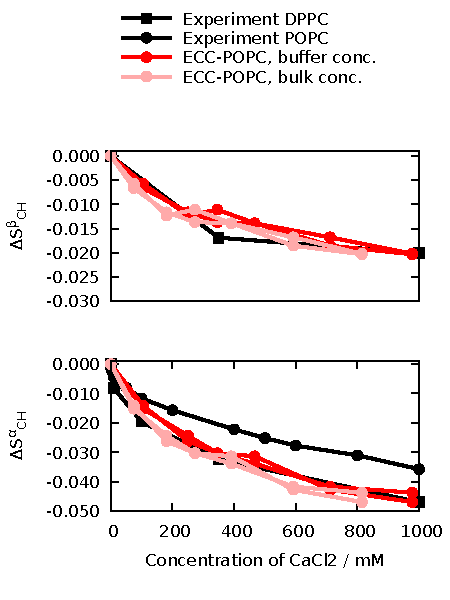
\includegraphics[width=8.3cm]{../Figs/OP_ECC_POPC_DPPC_water_conc2_dppc_bulk.pdf}
  \caption{\label{concentrationDEFfigure}
    Changes of the headgroup order parameters as a function of CaCl$_2$ concentration using
    two possible definitions of ion concentration from the recent force field
    with realistic calcium binding affinity to a POPC bilayer \cite{melcr18}
    together with the experimental data \cite{akutsu81,altenbach84}. 
  }
\end{figure}


\pagebreak
\section{Spectral slices in the indirect dimension from the R-PDLF and SDROSS experiments}

The C--H bond order parameters of the headgroup and glycerol backbone carbons are determined 
as $S_{\rm CH}=\Delta\nu/(0.315\times21.5  {\rm kHz})$, where $\Delta\nu$ is the dipolar splitting
given by the largest peak widths observed in the second dimension of the R-PDLF spectra
(blue lines in Fig. \ref{DPslices}), 0.315 is the scaling factor of the R18 recoupling sequence 
and 21.5~kHz is the maximum $^1$H--$^{13}$C dipolar coupling for a C--H bond \cite{dvinskikh04}.
%Slices of the R-PDFL spectra (Fig. \ref{DPslices}) 
%show a single splitting for the $\beta$-carbon with the order parameter value of 0.11,
%and a superposition of a large and a very small splitting for the $\alpha$-carbon.
%The larger splitting from the $\alpha$-carbon gives a order parameter value of 0.09, while the numerical value
%from the small splitting cannot resolved with the available resolution.
The resulting order parameters are in good agreement with the previously reported values
from $^2$H NMR experiments \cite{browning80} (Fig. \ref{HGorderParameters} in the main text).
However, the resolution in our $^{13}$C NMR experiment was not sufficient to detect the
the splitting related to the smaller order parameter of the C--H bond in the $\alpha$ carbon
observed in $^2$H NMR experiments \cite{browning80}. Therefore, the value of  0 $\pm$ 0.02 from our
$^{13}$C NMR experiments is shown figure \ref{HGorderParameters} 
and the magnitude of 0.02 from the literature is used in the SIMPSON calculations in the main text.

Interpretation of the order parameter signs of the $\alpha$ carbon from the SDROSS experiment
is complicated by the presence of distinct order parameters for the two attached hydrogens.
As discussed in the main text, interpretation of the SDROSS curve with the help of SIMPSON
simulations gave values $+0.09$ and $-0.02$ for the $\alpha$-carbon order parameters.
To corroborate our interpretation, we measured the SDROSS curve also using the higher 8~kHz
MAS frequence (Fig. \ref{DPslices} bottom), which makes the experiment more sensitive to larger order parameter values.
Also this experiment indicates a positive value for the larger $\alpha$-carbon order parameter.
\begin{figure}[]
%  \centering
  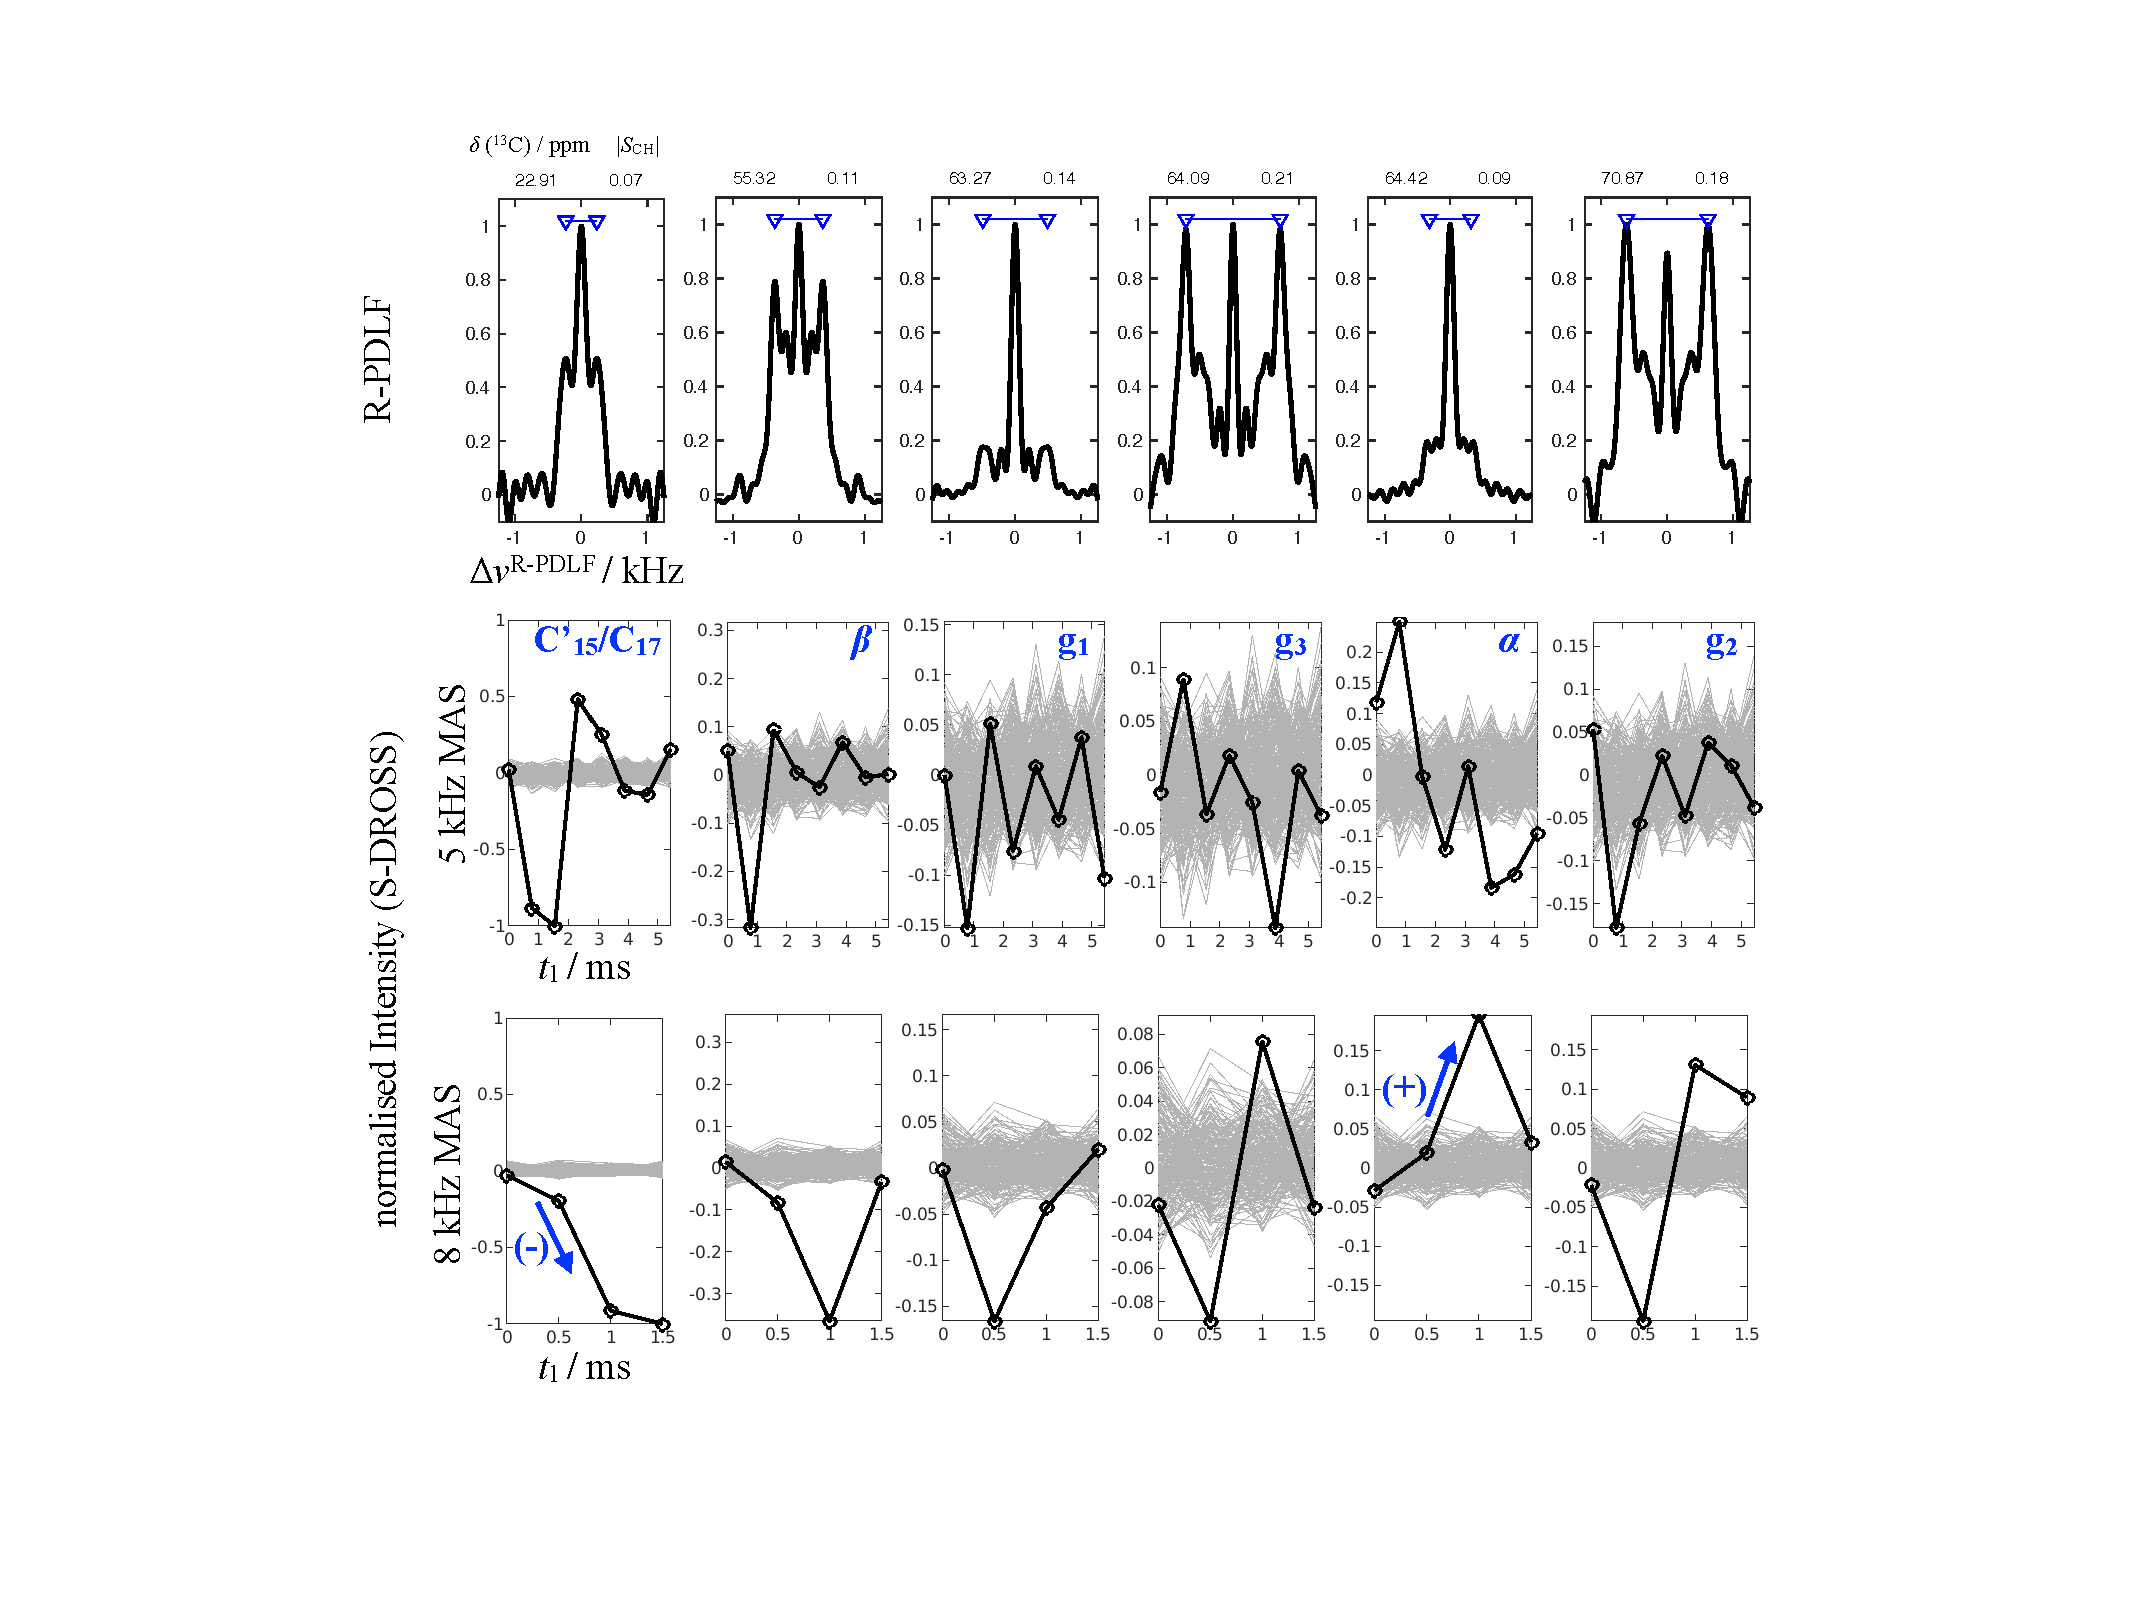
\includegraphics[width=\textwidth]{../Figs/SI_man.pdf}
  \caption{\label{DPslices}
    Spectral slices in indirect dimension from the R-PDLF (top) and S-DROSS (middle and bottom) experiments at distinct chemical shifts.
    The chemical shifts and order parameters (calculated from the dipolar splittings indicated with blue lines in the R-PDLF slices)
    are shown on top each column (chemical shift left, order parameter right).
    The assignment of columns is given in the middle.  
    The SDROSS slices were measured using both 5~KHz (middle) and 8~kHz (bottom) because different MAS frequencies enable the
    higher sensitivity to the order parameters with lower and higher magnitudes, respectively.
    The background noise taken from chemical shift slices without carbon peaks (grey lines in SDROSS figures)
    are used to determine the error bars for $\alpha$ and $\beta$ carbons in Fig.~\ref{PShgSIGNSsimpson} in the main text.
    The SDROSS profile of the acyl chain methyl carbons (left column) was used as reference assuming that these carbons have negative order parameters.  
  }
\end{figure}

\pagebreak
\section{Dihedral angle distributions of the headgroup and glycerol backbone
  regions of PS lipids from different simulation models}\label{Diheds}

The dihedral angles and structures of the glycerol backbone and headgroup regions of POPS lipids show
wide variety between different simulation models (Figs.~\ref{dihedralsHG}, \ref{dihedralsGLY} and \ref{HGandGLYstructuresPS}).
Detailed discussion of the structural differences is limited by the lack of realistic model that would correctly reproduce the
headgroup and glycerol backbone order parameters. However, some structural characteristics
of PS headgroup can be suggested based on the best available models
(Figs.~\ref{dihedralsHGpc}, \ref{dihedralsGLYpc} and \ref{HGandGLYstructuresPSPC}), as discussed in the main text.
The glycerol backbone structures are not discussed in this work because our focus is on PS headgroup.
However, the data presented here can be useful for future investigations.
%backbone order parameters of C$_2$ and C$_3$ from Slipids simulations
%differ significantly from the other simulation results and experiments (Fig. \ref{HGorderParametersPS}),
%as observed previously also for PC lipids \cite{botan15}.
%The origin of this difference is more difficult to track without more elaborate analysis,
%because different models show very complicated patterns of distinct structures
%in the glycerol backbone region (Figs.~\ref{HGstructuresPS} and \ref{dihedralsHG}).

\begin{figure*}[]
  \centering
  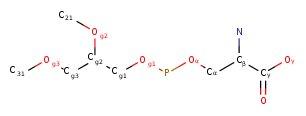
\includegraphics[width=8.0cm]{../Figs/PS_Labels.png}
  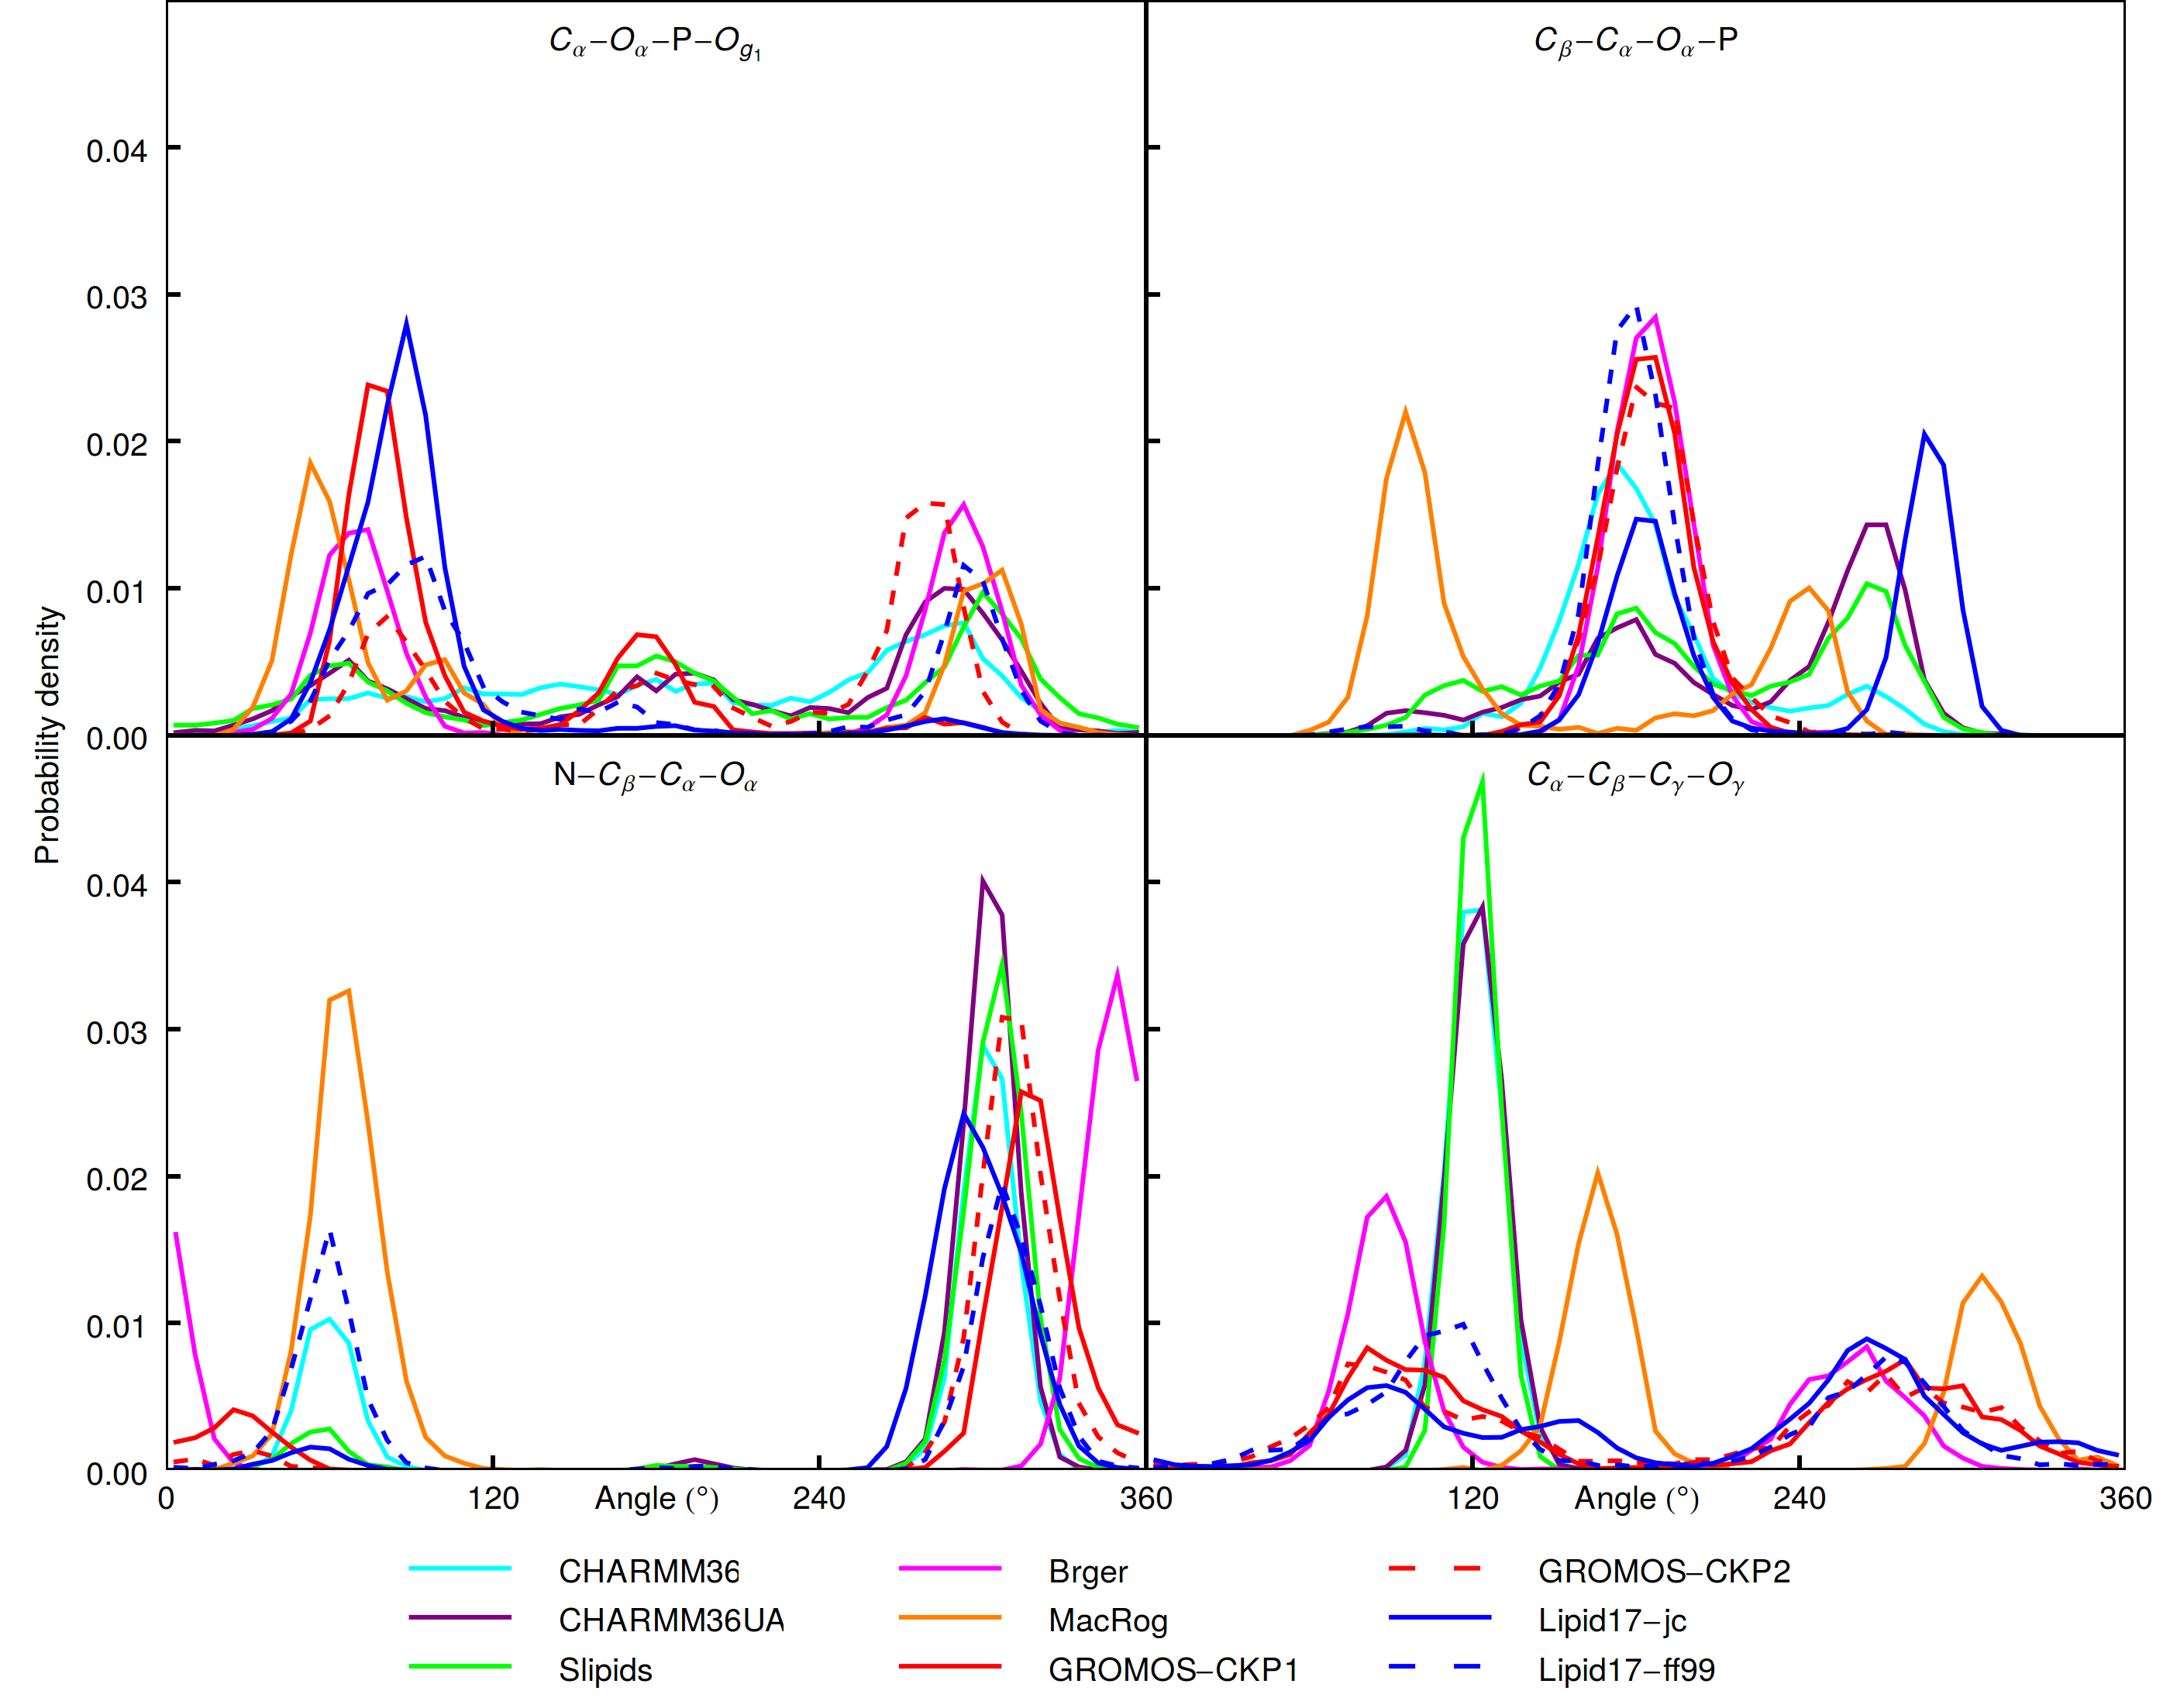
\includegraphics[width=16.0cm]{../Figs/figS7.png}
  \caption{\label{dihedralsHG}
    Dihedral angle distributions of the headgroup region of POPS from different simulation models.
  }
\end{figure*}

\begin{figure*}[]
  \centering
    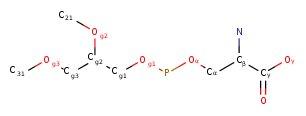
\includegraphics[width=8.0cm]{../Figs/PS_Labels.png}
  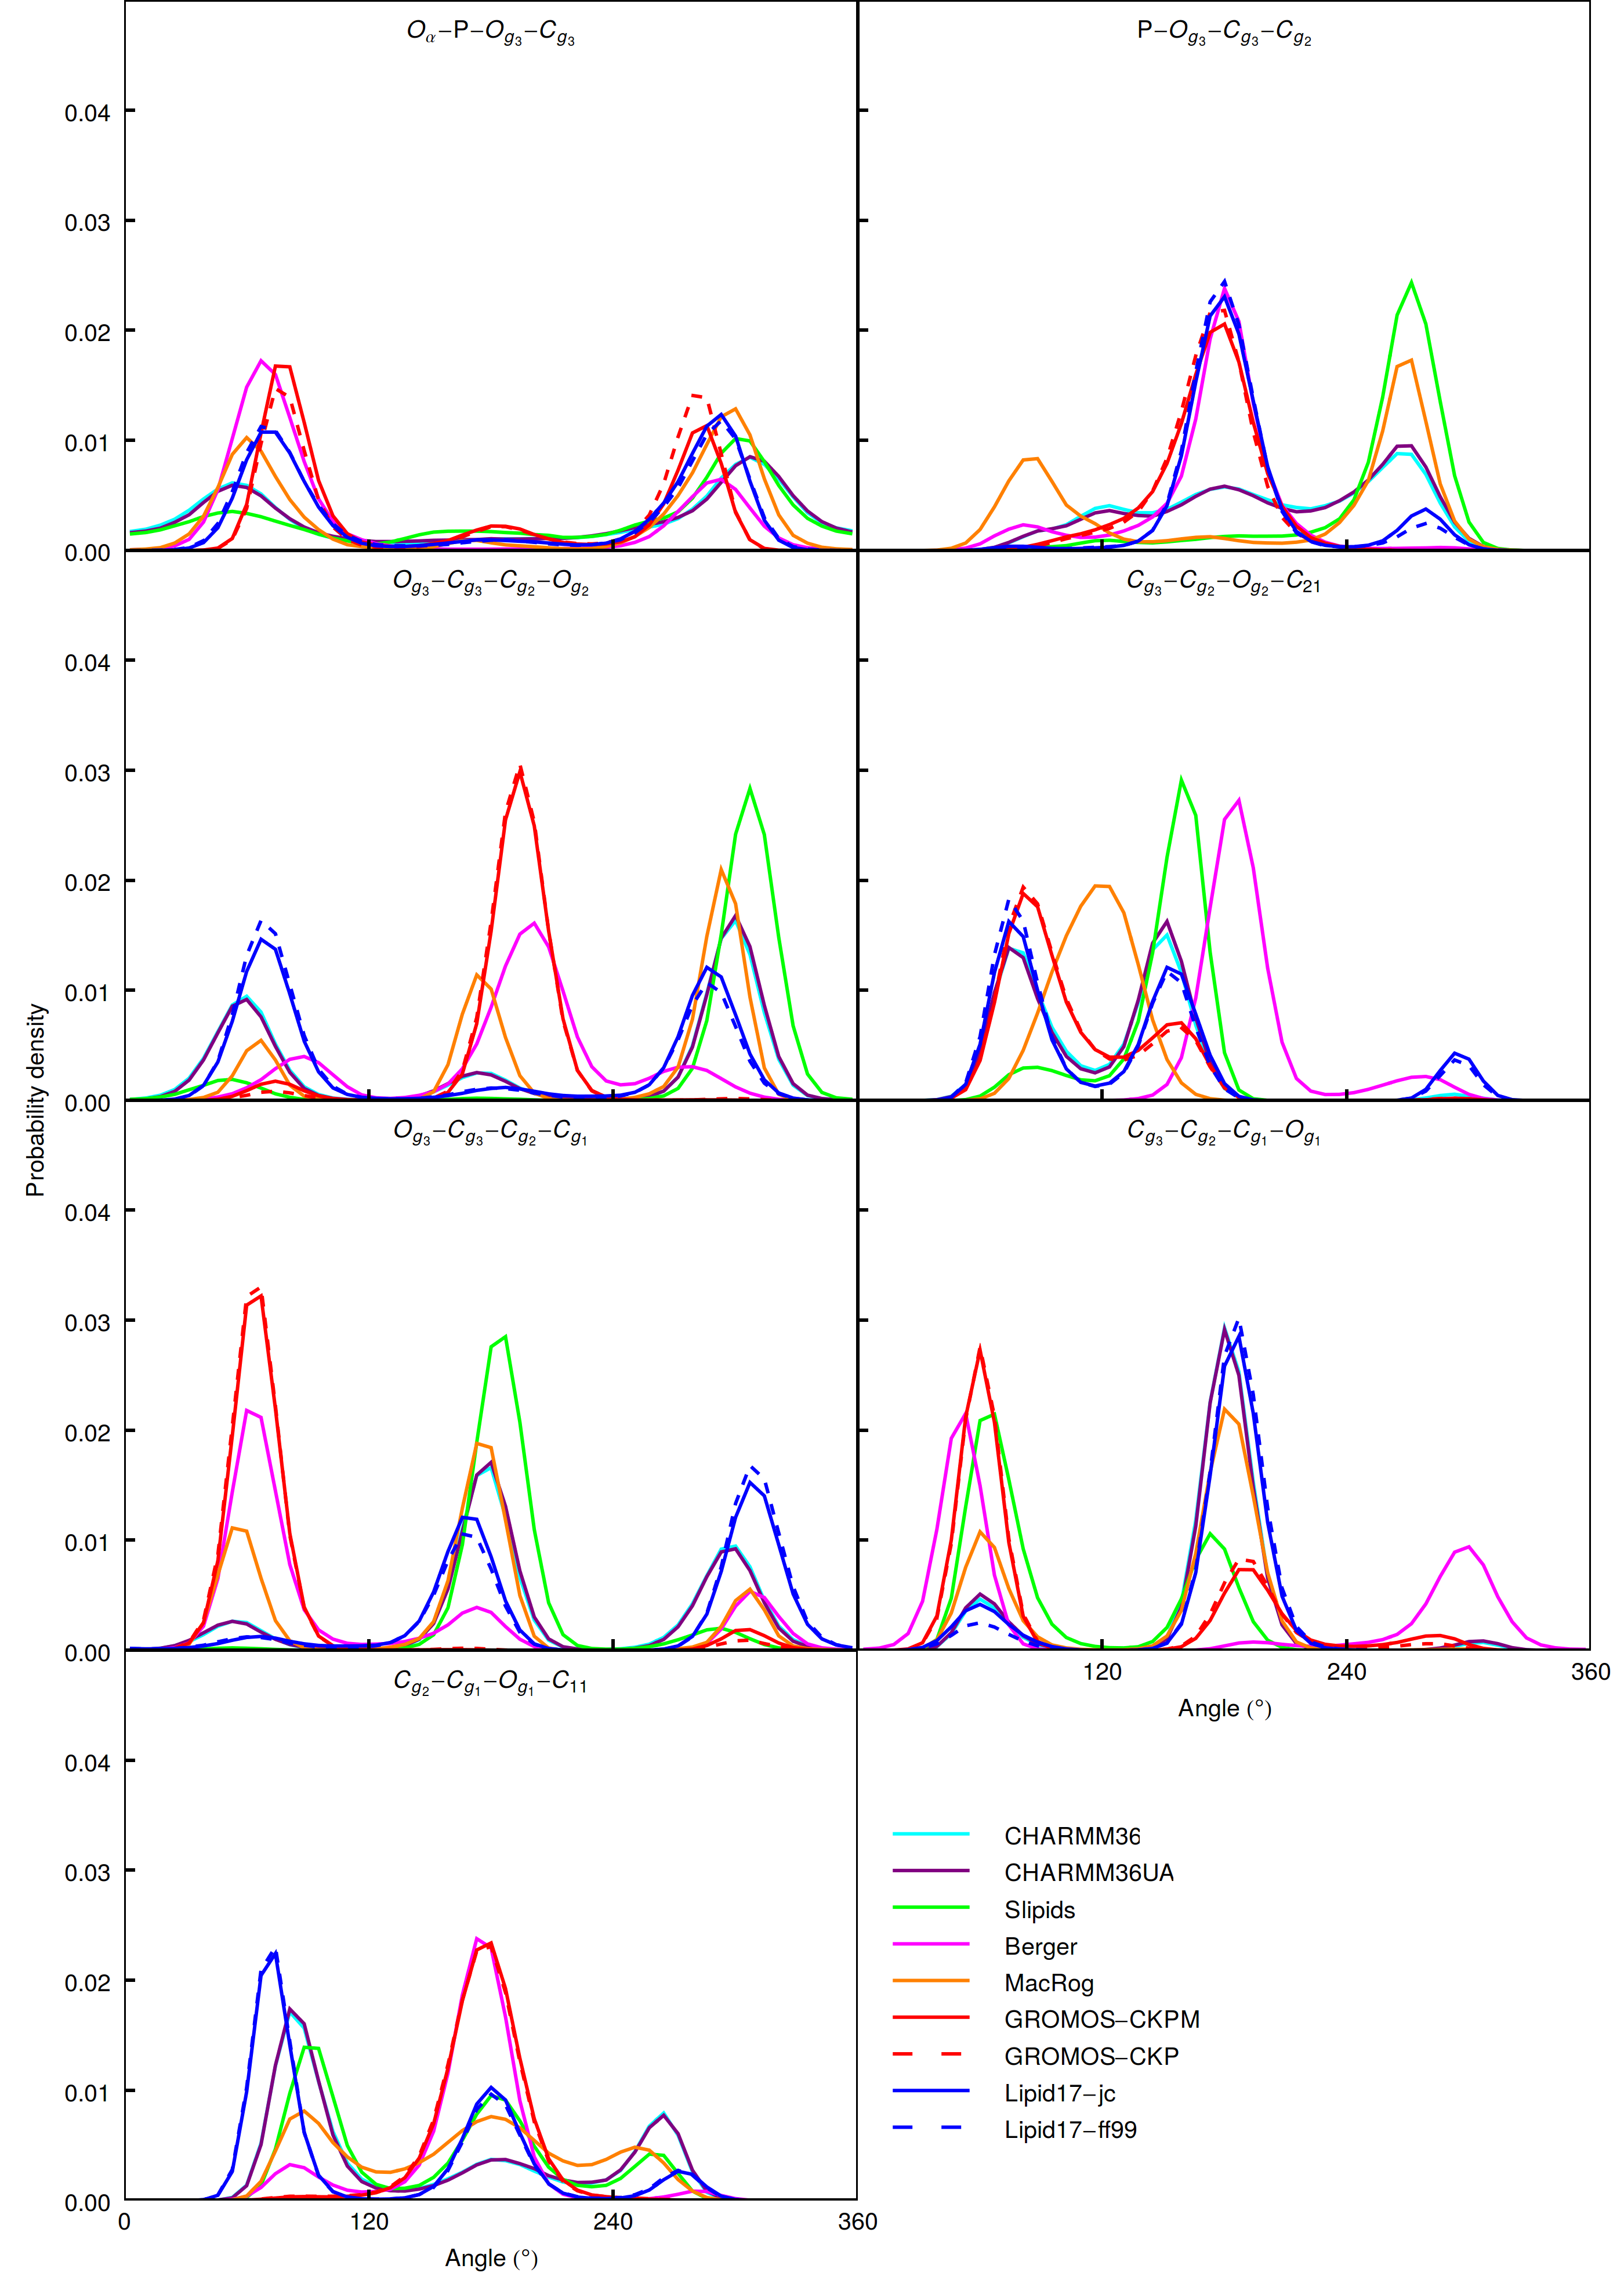
\includegraphics[width=13.0cm]{../Figs/figS6.png}
  \caption{\label{dihedralsGLY}
    Dihedral angle distributions of the glycerol backbone region of POPS lipids from different simulation models.
  }
\end{figure*}

\begin{figure*}[]
  \centering
  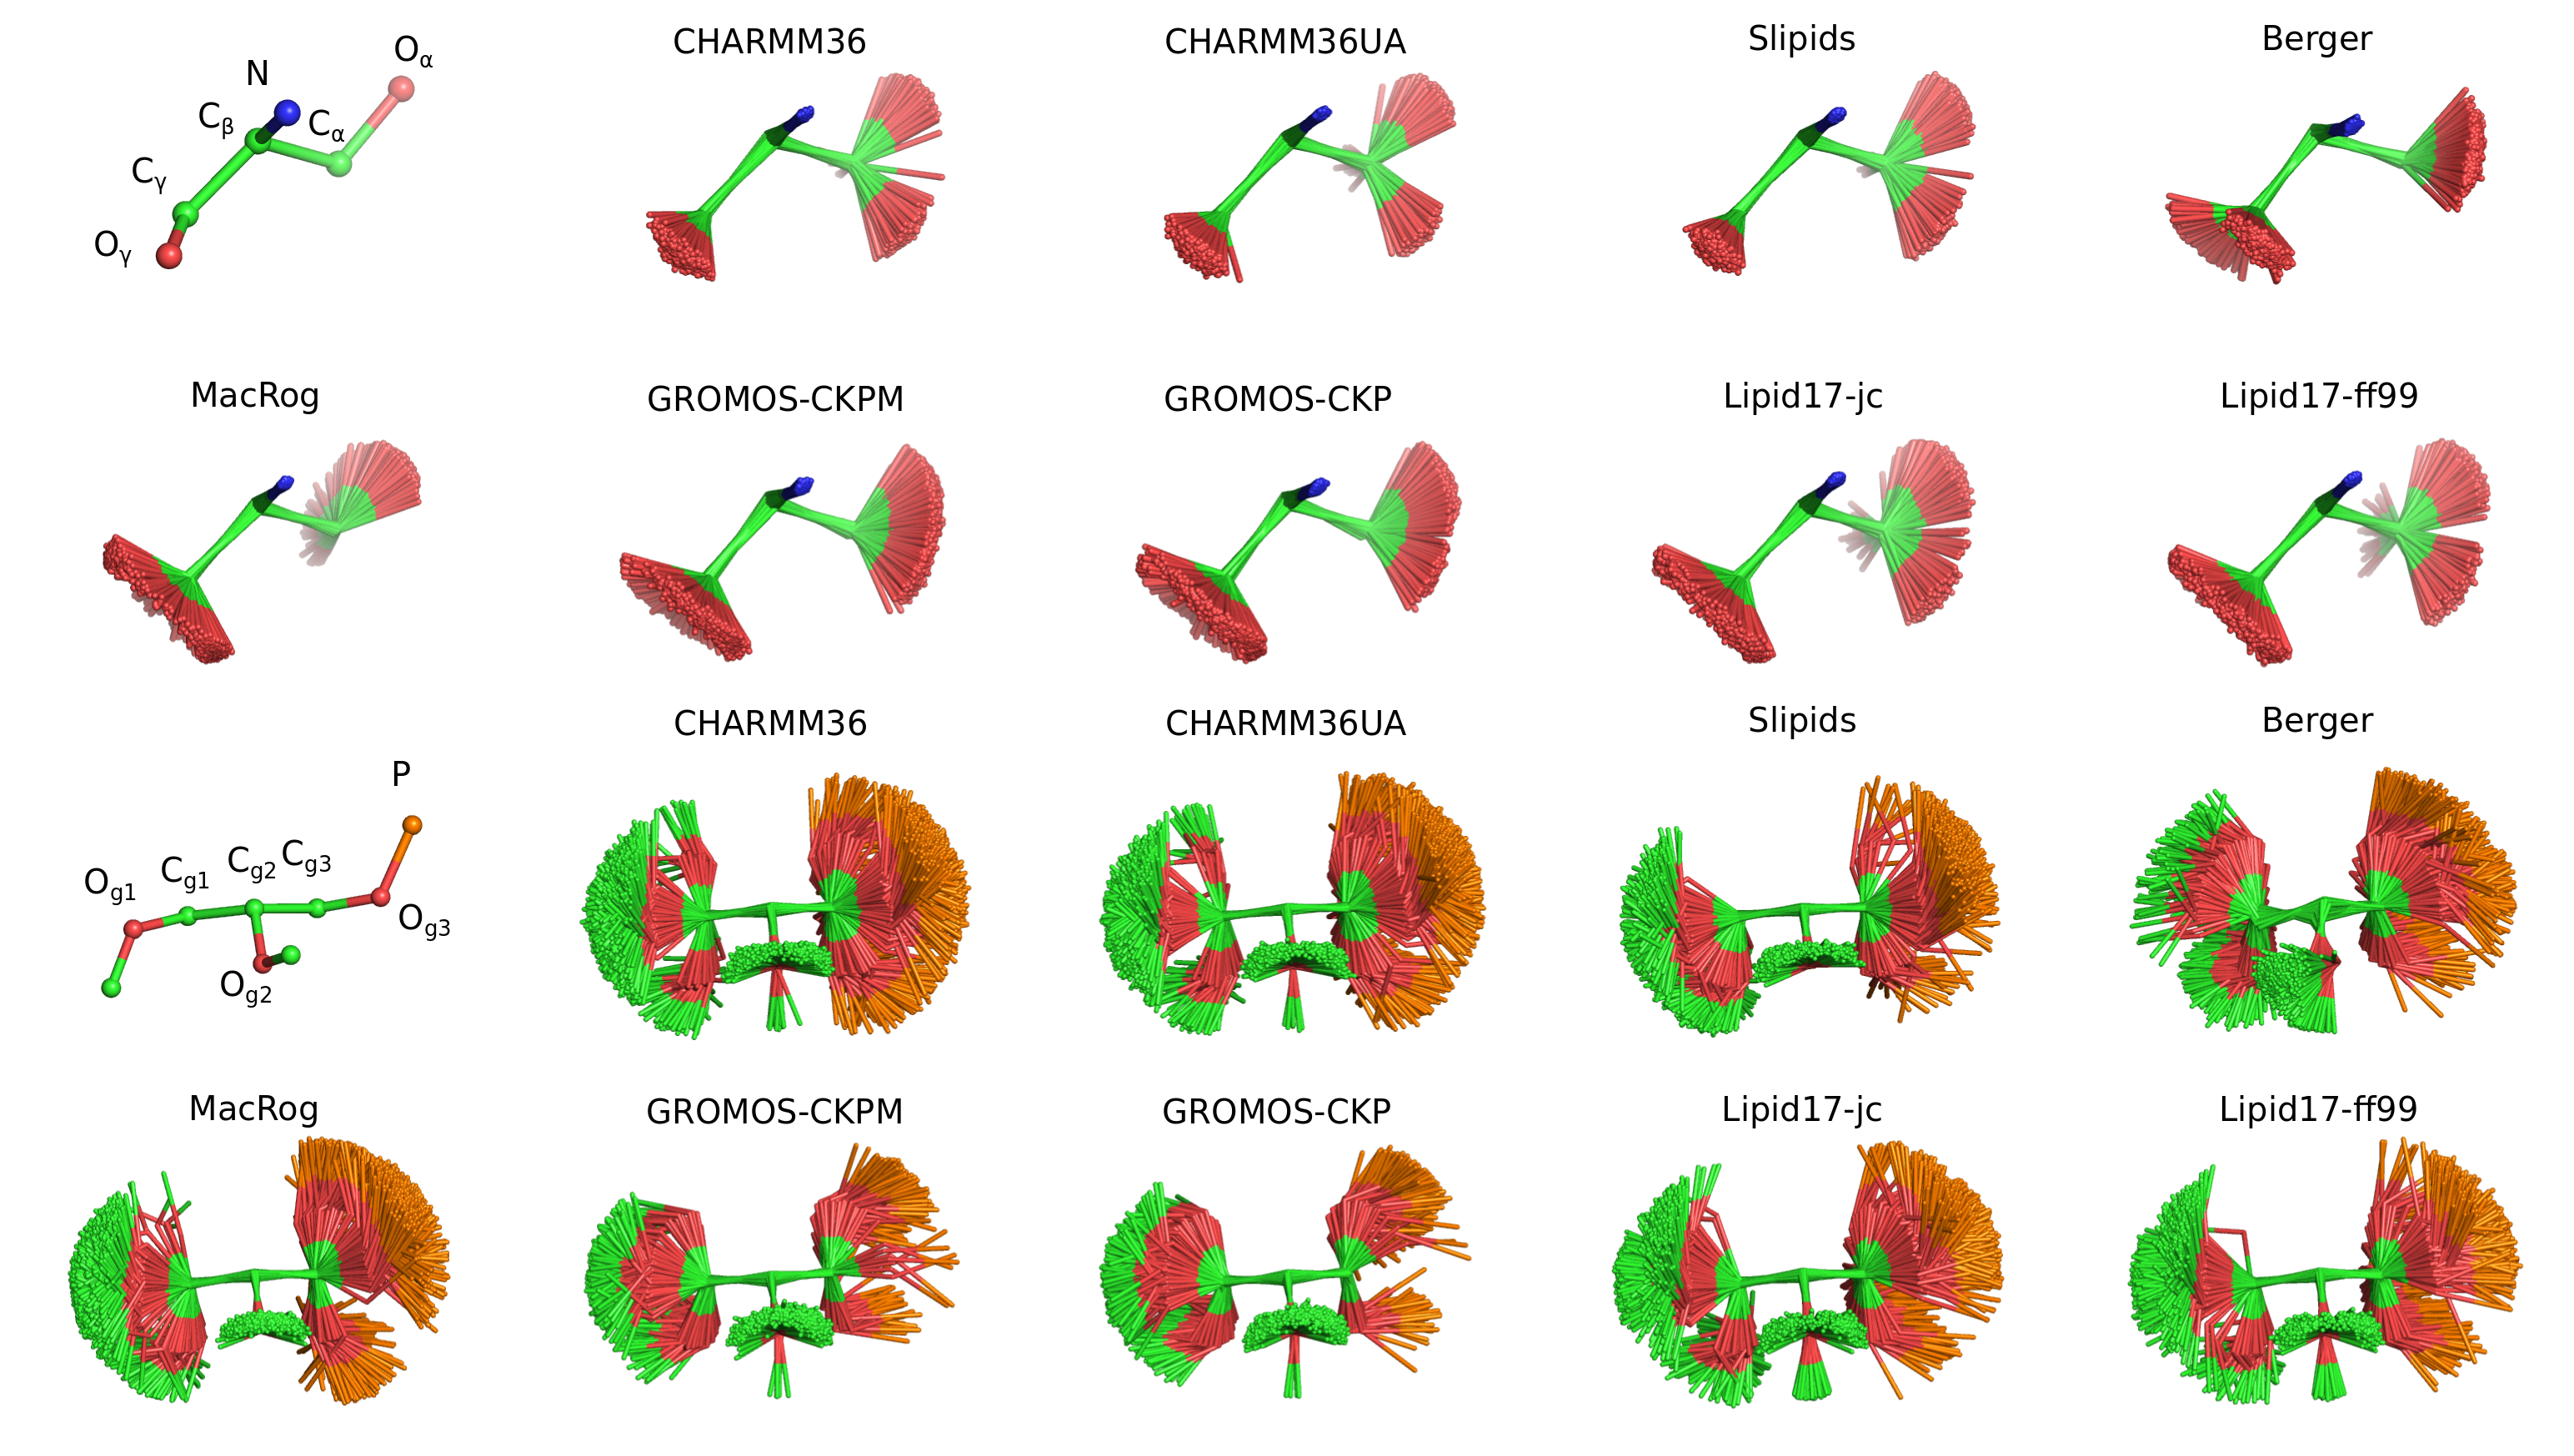
\includegraphics[width=18.0cm]{../Figs/figS8.png}
  \caption{\label{HGandGLYstructuresPS}
    Overlayed snapshots of the glycerol backbone and headgroup regions from different POPS simulations.
  }
\end{figure*}

\begin{figure*}[]
  \centering
  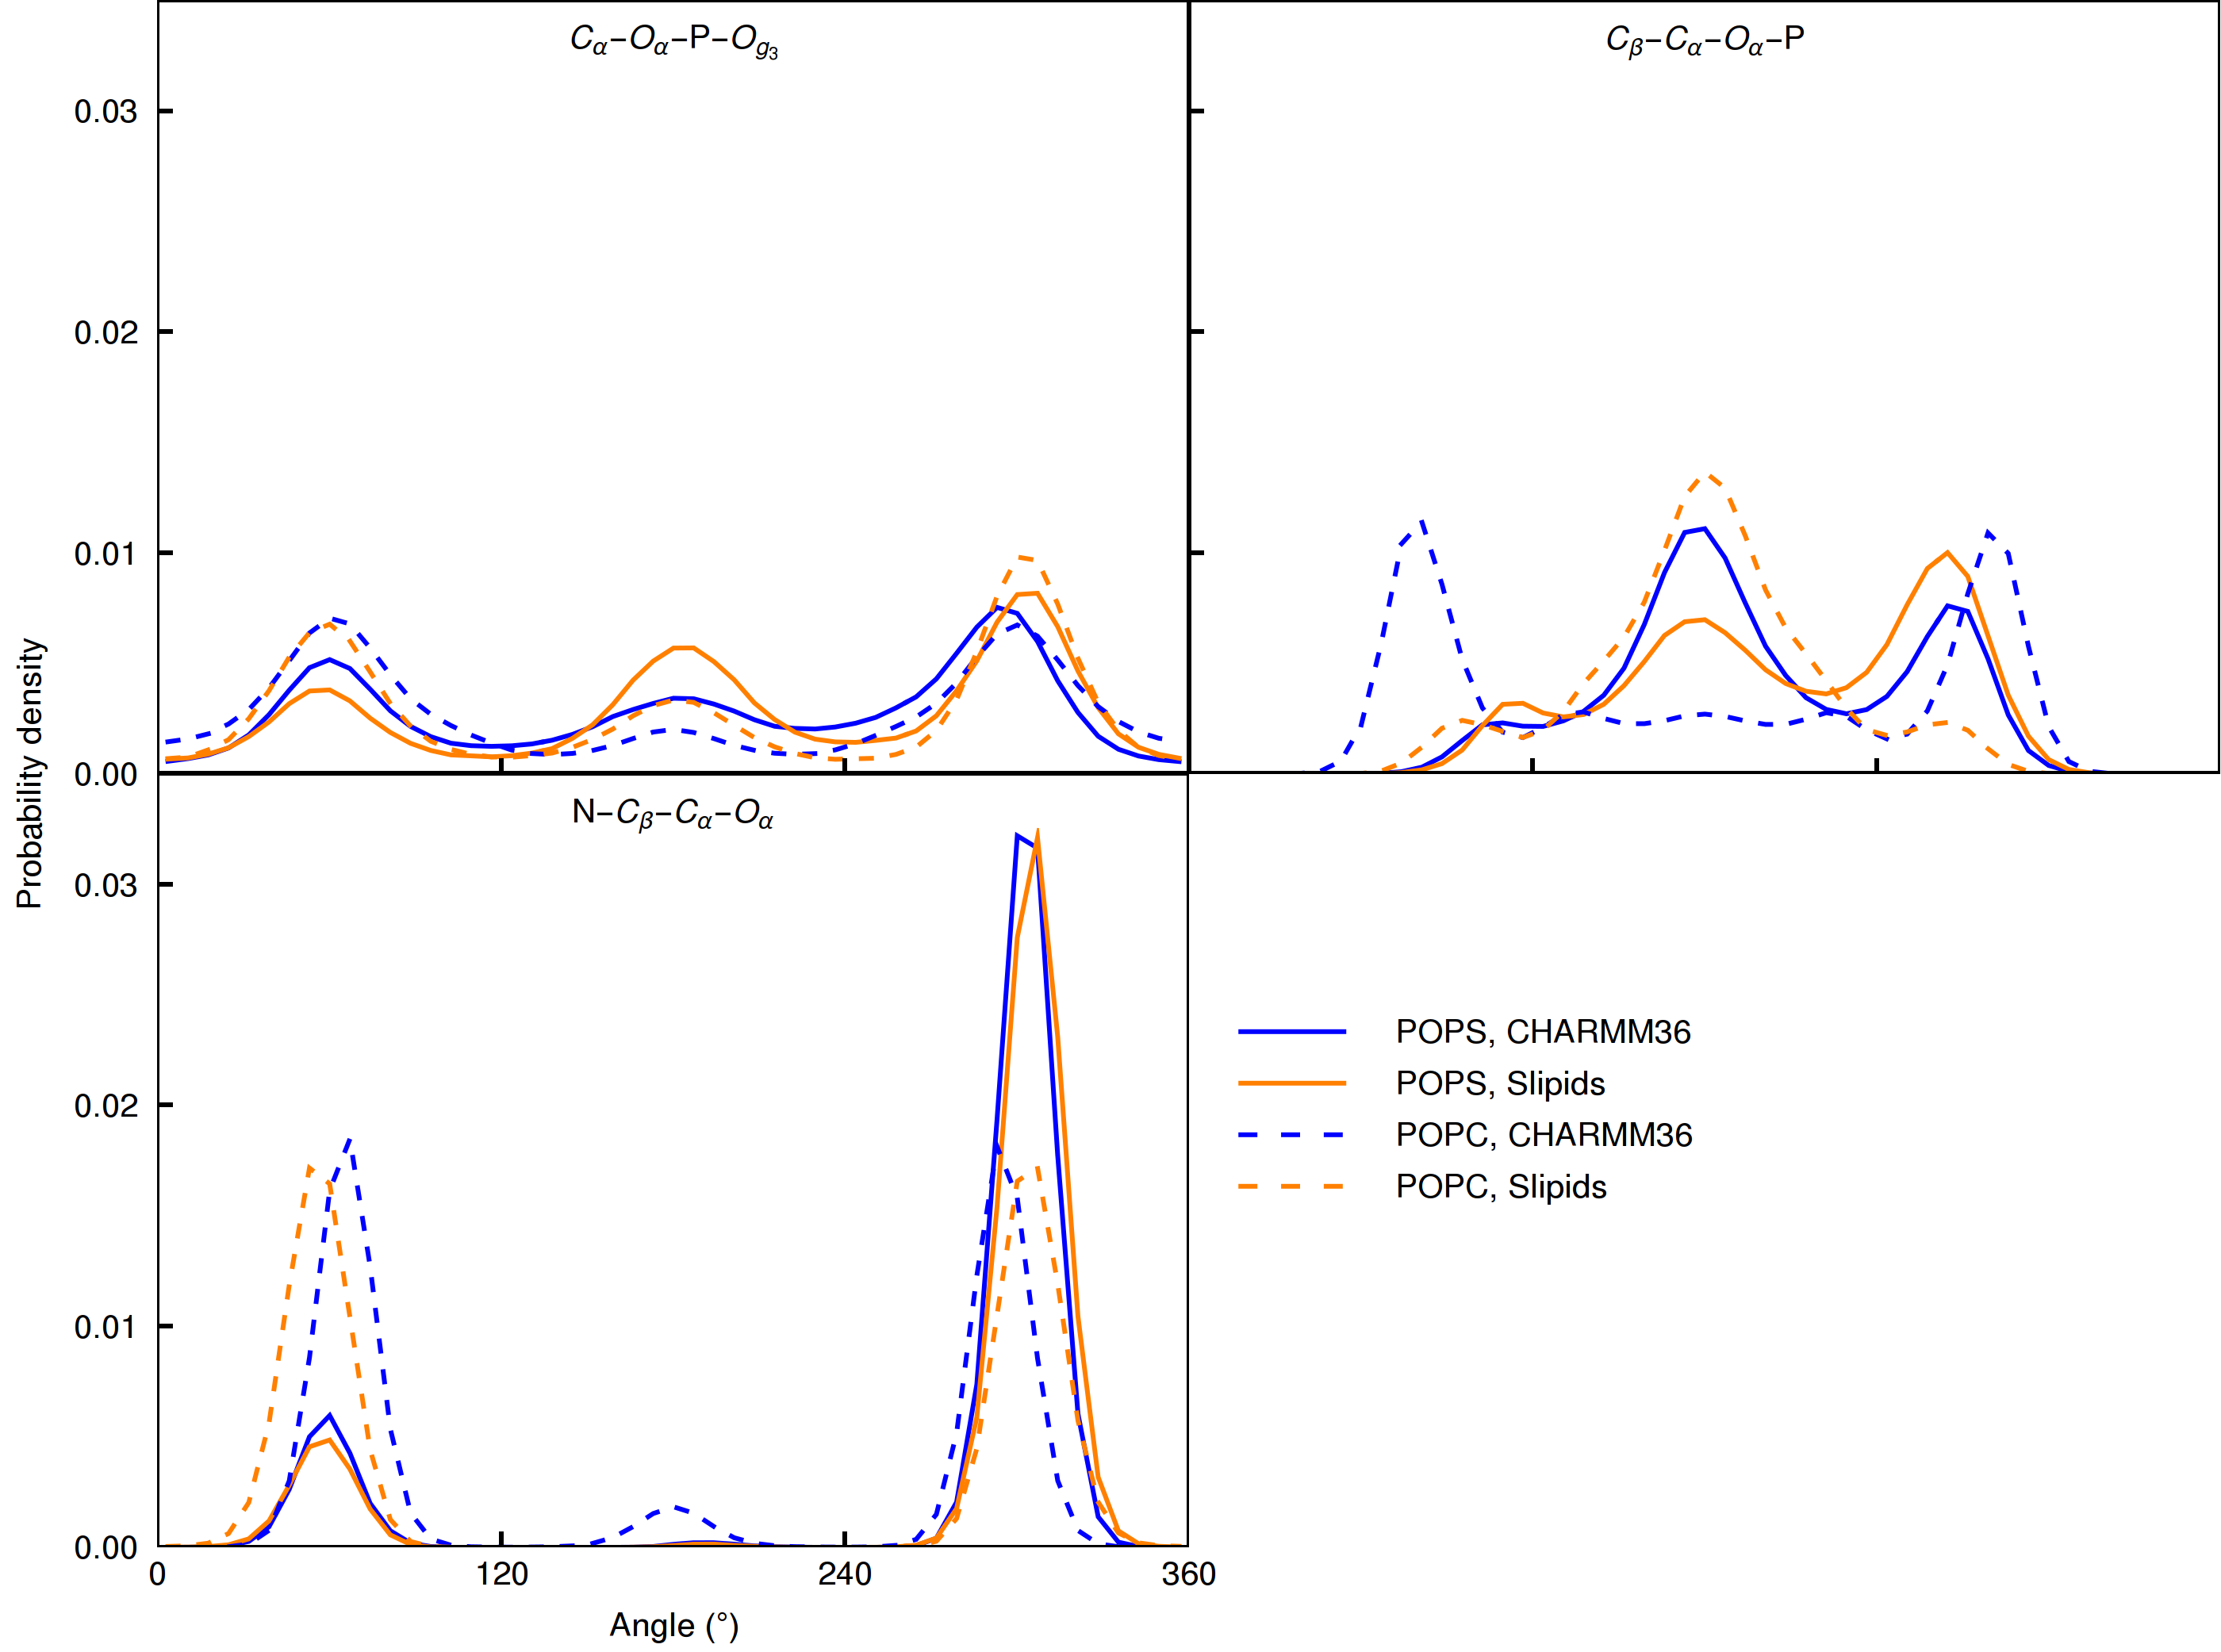
\includegraphics[width=16.0cm]{../Figs/figS11.png}
  \caption{\label{dihedralsHGpc}
    Dihedral angle distributions of the headgroup regions from CHARMM36 and Slipids simulations
    compared between the POPC and POPS lipids. 
    The CHARMM36 POPC simulation is from Ref.~\citenum{POPCcharmm36T303K} and Slipids POPC from Ref.~\citenum{POPCslipids298K}.
  }
\end{figure*}

\begin{figure*}[]
  \centering
  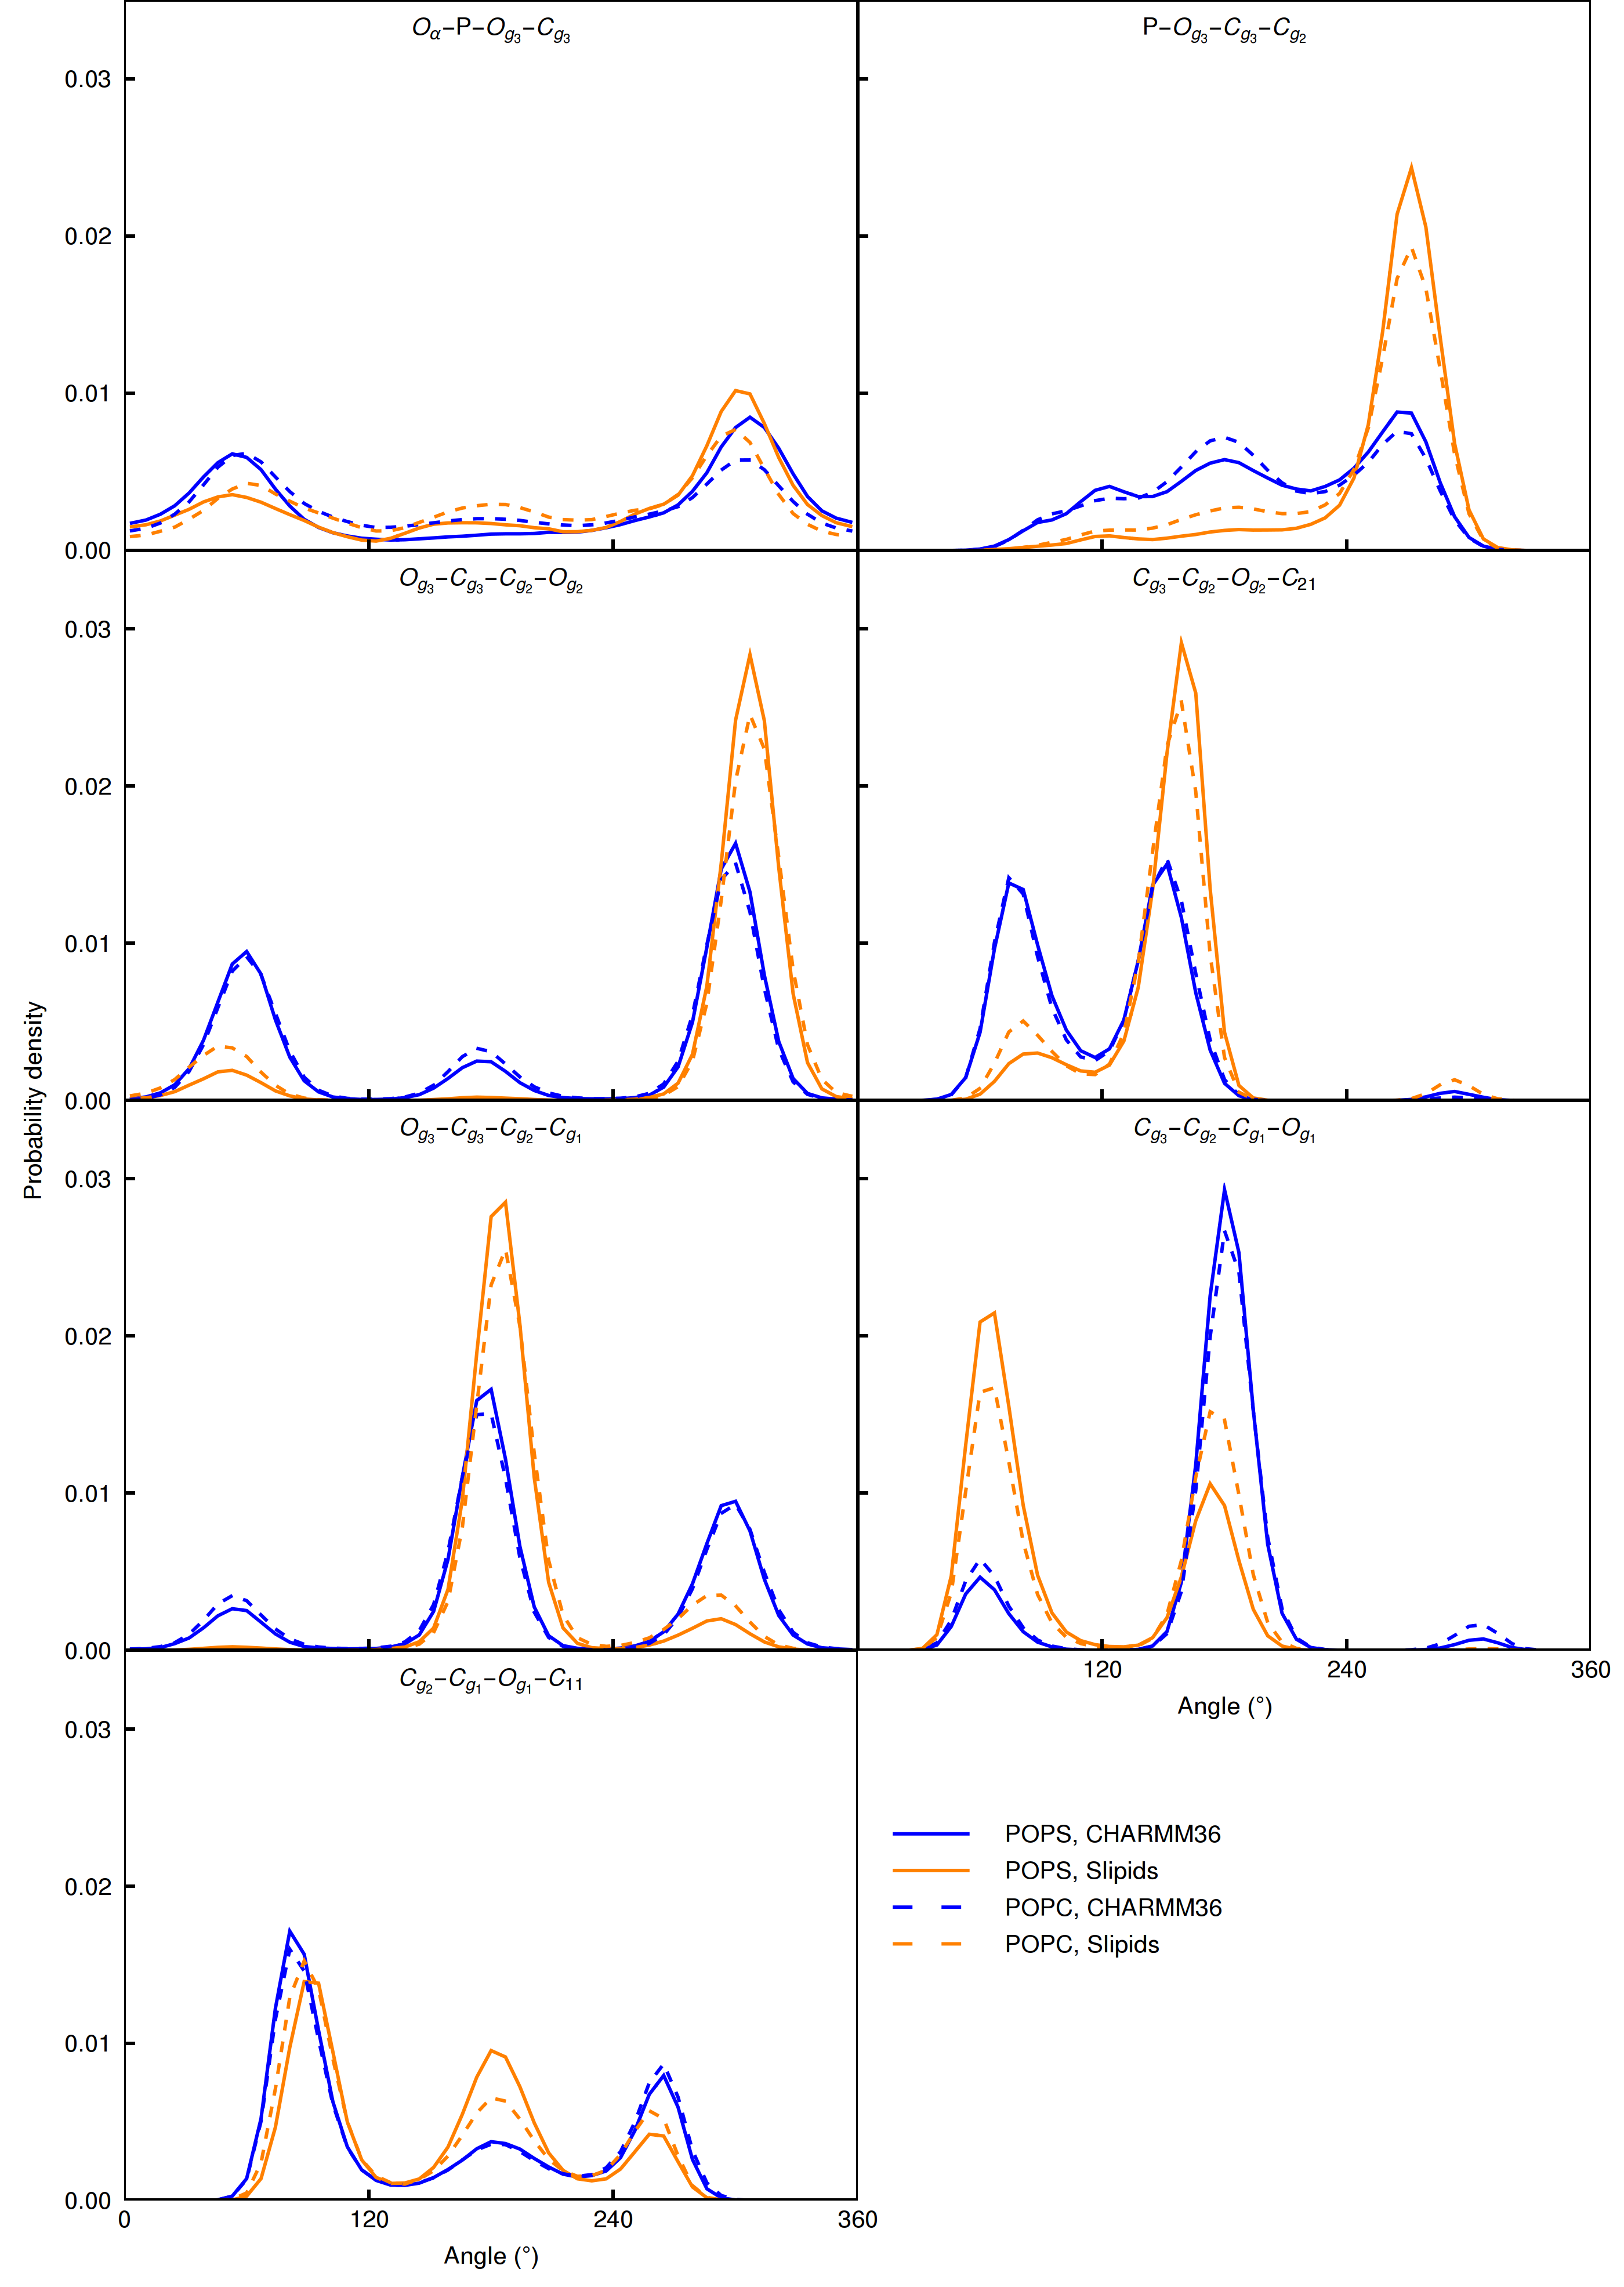
\includegraphics[width=15.0cm]{../Figs/figS10.png}
  \caption{\label{dihedralsGLYpc}
    Dihedral angle distributions of the glycerol backbone regions from CHARMM36 and Slipids simulations
    compared between the POPC and POPS lipids.
    The CHARMM36 POPC simulation is from Ref.~\citenum{POPCcharmm36T303K} and Slipids POPC from Ref.~\citenum{POPCslipids298K}.
  }
\end{figure*}

\begin{figure}[]
  \centering
  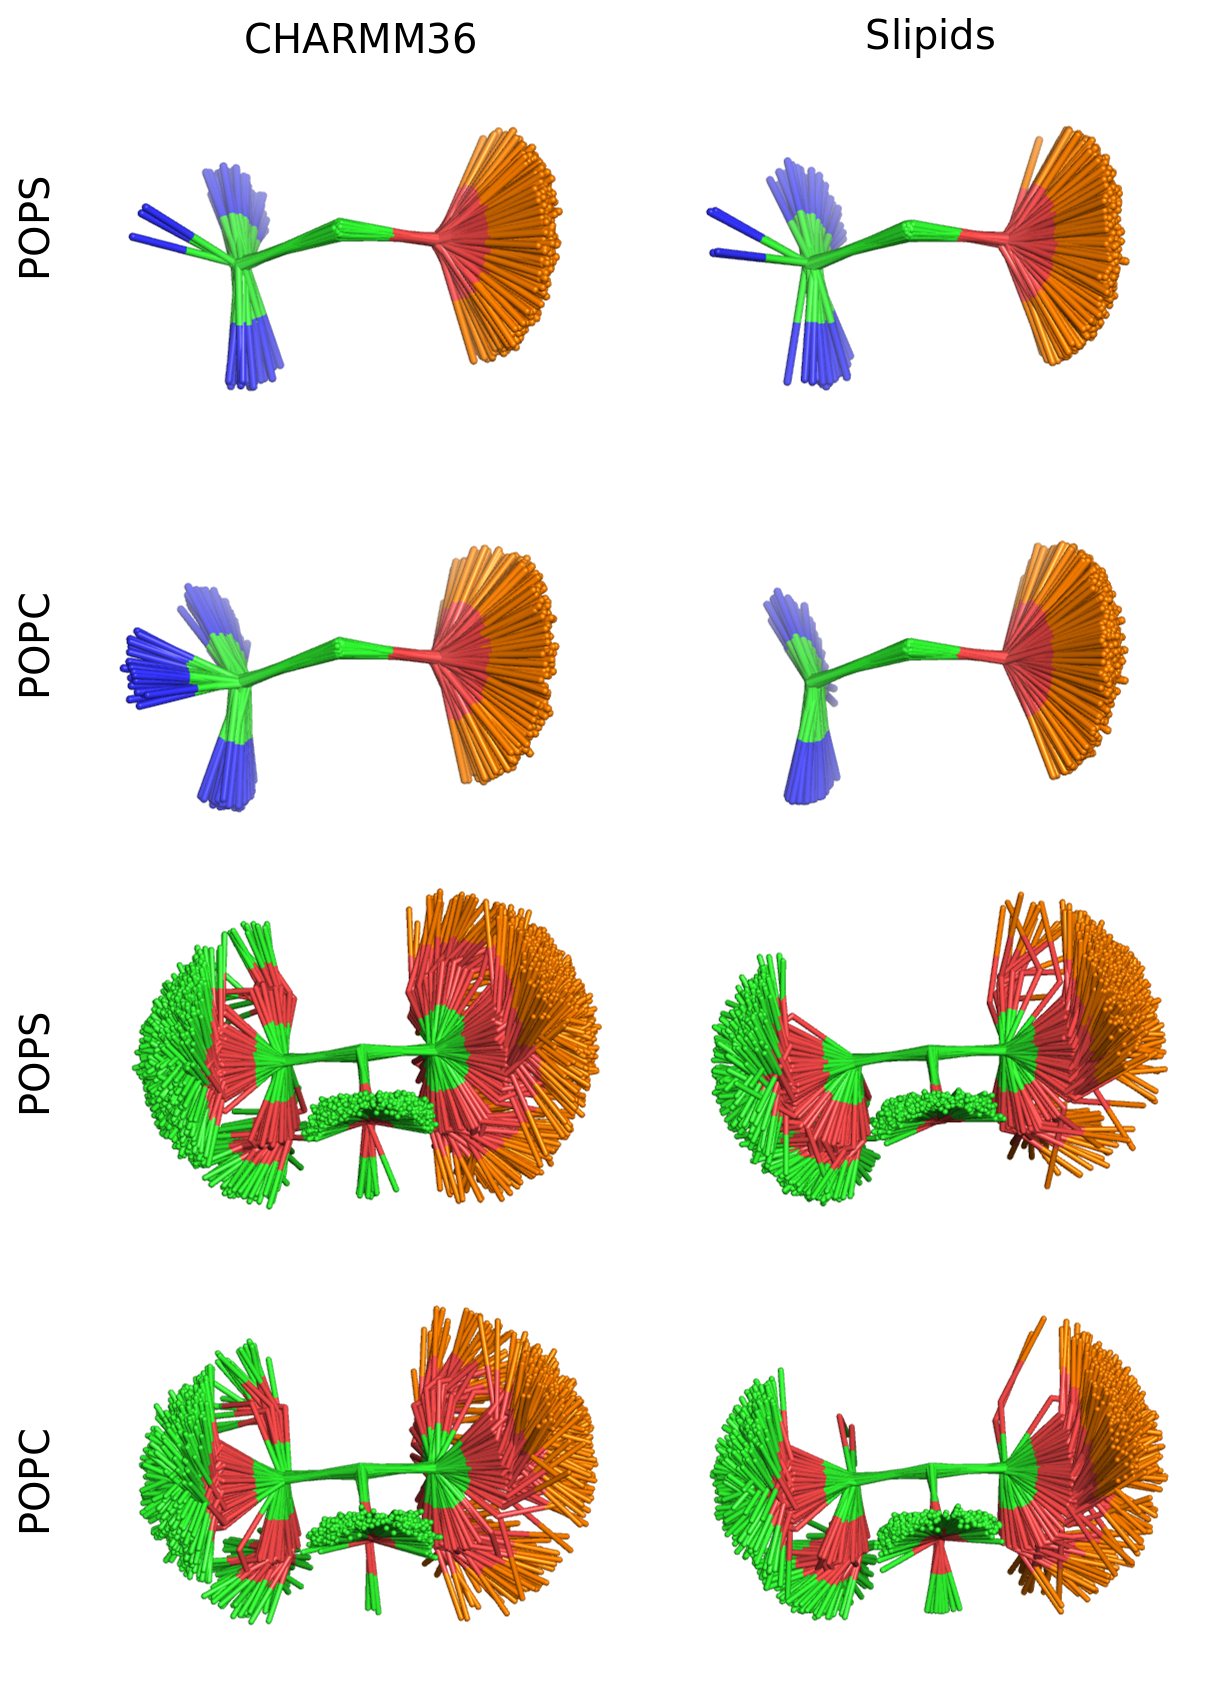
\includegraphics[width=9.0cm]{../Figs/figS8_POPC.png}
  \caption{\label{HGandGLYstructuresPSPC}
    Overlayed snapshots of the headgroup and glycerol backbone regions 
    from CHARMM36 and Slipids simulations compared between the POPC and POPS lipids.
    The CHARMM36 POPC simulation is from Ref.~\citenum{POPCcharmm36T303K} and Slipids POPC from Ref.~\citenum{POPCslipids298K}.
  }
\end{figure}




\pagebreak

\section{Headgroup response to the additional counterions in POPC:POPS (5:1) mixtures}\label{mixtureTOadditionalCIs}
To evaluate counterion binding in different simulation models against experimental data~\cite{roux90},
we plot the headgroup order parameters measured from POPC:POPS 5:1 mixture
as a function of different monovalent ions added to the buffer (Fig.~\ref{PSresponseTONaCl}). 
Experimental order parameters of POPC headgroup in the mixture are available as a function
of LiCl and KCl concentrations, while POPS headgroup order parameters are measured also
in increasing NaCl concentration. Lithium interacts more strongly with PS headgroups than other monovalent 
ions~\cite{hauser83,hauser85,roux86,mattai89,roux90}, as also observed for PC headgroups~\cite{cevc90}. 
The different binding behaviour is evident based on the response of PS headgroup order parameters, which decrease with the addition of lithium 
but increase with the addition of sodium or potassium (Fig.~\ref{PSresponseTONaCl}). 
POPC headgroup order parameters exhibit a clear decrease as a function of LiCl concentration
but only modest changes as a function of KCl concentration, indicating singificant 
Li$^+$ binding but only weak K$^+$ binding to the mixture when interpreted using the
electrometer concept~\cite{akutsu81,altenbach84,seelig87}.

In simulations with Berger and CHARMM36 models, the responses of POPC and POPS order parameter
to added sodium and potassium are not in line with the experiments. Instead, the simulations produces a response similar to experiments conducted in LiCl (Fig.~\ref{PSresponseTONaCl}), indicating overestimated binding affinity of sodium and potassium 
in these simulations. The MacRog simulations with potassium exhibit weaker counterion binding affinity
(Fig.~\ref{CIdensPSOCmixt}), but significantly larger error bars and
less systematic changes in the order parameters (Fig.~\ref{PSresponseTONaCl}).
Similar unsystematic behaviour was also observed in the simulations of Lipid14/17 model
with the additional counterions \cite{POPCpopsLIPID17withKCI,POPCpopsLIPID17withK,POPCpopsLIPID17withNaCI,POPCpopsLIPID17withNa},
for which the data is not shown due to the formation of
ion clusters in water with relatively low (1~M) ion concentrations (Fig.~\ref{ionCLUSTERS}).
Appearance of such clusters in the MagRog simulations with 4~M KCl
could explain the unsystematic changes of the order parameters in this model upon increasing KCl.
In conclusion, the results are in line with the Section \ref{ciBINDINGsection}
in the main text, suggesting that the MacRog simulations with KCl give the most
realistic surface charge at the lipid bilayer interface among the tested simulation models.
\begin{figure*}[]
  \centering
  \includegraphics[width=17.0cm]{../Figs/CHANGESwithMONVALENTwithPS.eps}
  \caption{\label{PSresponseTONaCl}
    Changes of the PC (left) and PS (right) headgroup order parameters as a function of
    added NaCl, KCl and LiCl from POPC:POPS (5:1) mixture at 298~K
    (except Berger simulations are (4:1) mixture at 310~K).
    The experimental data is from Ref.~\citenum{roux90}.
    The values from counterion-only systems are set as a zero point of y-axis.
    To correctly illustrate the significant forking of the $\alpha$-carbon order parameter
    in PS headgroup (bottom, right), the y-axis is shifted with the same value for both order parameters such that the lower order
    parameter value is at zero.
  }
\end{figure*}
\begin{figure}[]
  \centering
  \includegraphics[width=8.0cm]{../Figs/CIdensPSOCmixt.eps}
  \caption{  Counterion density distributions from PC:PS mixtures.
\label{CIdensPSOCmixt}
  }
\end{figure}
\begin{figure}[]
  \centering
  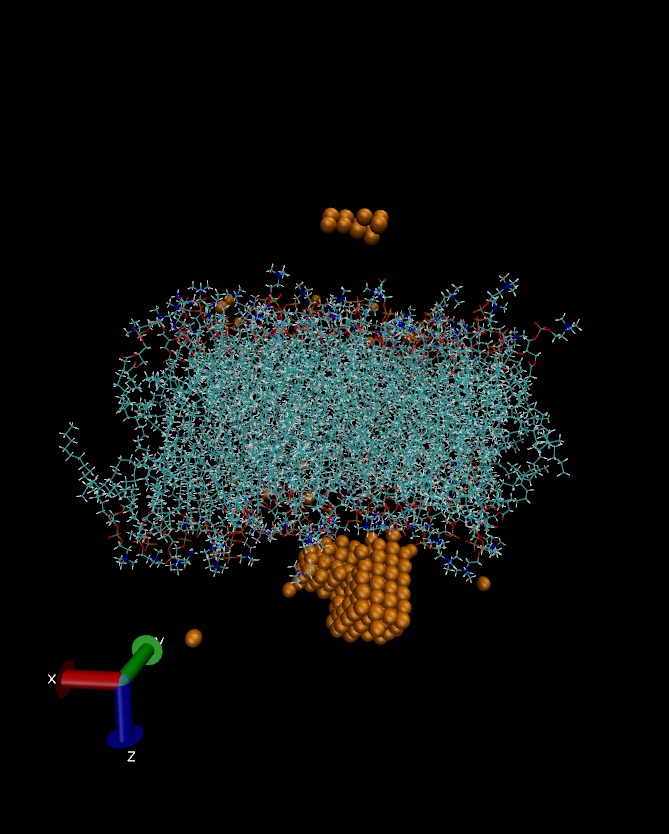
\includegraphics[width=8.0cm]{../Figs/lipid17cluster.png}
  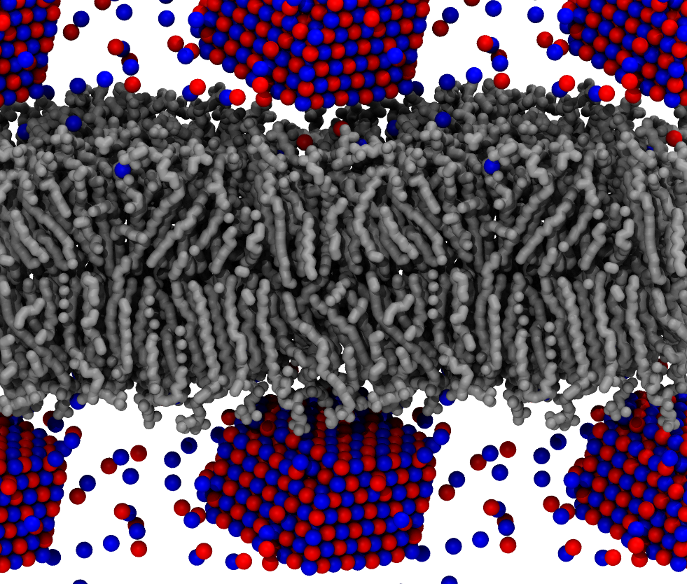
\includegraphics[width=8.0cm]{../Figs/MacRogIONcluster.png}
  \caption{Ion clusters appearing in POPC:POPS (5:1) lipid17/14 simulations with 1~M of NaCl (left)
    and MacRog simulations with 4~M of KCl (right).
\label{ionCLUSTERS}
  }
\end{figure}
\newpage

%%
%% I think that this section is not very useful, I think that we should remove it.
%%
%\section{Sodium binding to DMPC:DOPS mixture}
%
%\begin{figure}[]
%  \centering
%  \includegraphics[width=9.0cm]{../Figs/PSresponseTONaCl.eps}
%  \caption{\label{PSresponseTONaClDMPC}
%    Order parameters of PS headgroup as a function of added NaCl measured from DMPC:DMPS (3:1) mixture \cite{roux86}.
%  }
%\end{figure}
%The experimental results show essentially no changes in the order parameters as a function of
%added NaCl, while significant changes are observed in simulations. However,
%the minimum buffer concentration of NaCl in the experimental was 100mM \cite{roux86}.
%Therefore, we cannot exclude the possibility that the NaCl induced changes were already
%saturated with 100mM NaCl concentration, which was the case for CaCl$_2$ in Fig. \ref{changesWITHCaClPS}.

\section{Calcium binding to POPC in CHARMM36 simulation with NBfix}\label{CHARMMcalciumNBfix}

The response of POPC headgroup order parameters to the CaCl$_2$ concentration
are underestimated in simulations of POPC:POPS (5:1) mixture with CHARMM36 when employing NBfix (as obtained from CHARMM-GUI in January 2018) for interactions between calcium and lipid oxygens \cite{kim16}
(Fig.~\ref{changesWITHCaClPS} in the main text),
indicating that the calcium binding to the bilayer is too weak with these
parameters. The response of headgroup order
parameters (Fig.~\ref{OP_CHARMM_CaCl_POPC_NBFix}) and the binding affinity
(Fig.~\ref{density_profile_CHARMM_CaCl_POPC_NBFix}) of calcium also to a pure
POPC bilayer are underestimated when using NBfix ions.  Notably, CHARMM36 simulations with the NBfix
terms \cite{venable13,kim16} predict similar binding affinity for sodium and calcium. Without the NBfix term, the calcium binding affinity to pure POPC lipid bilayers was overestimated in the CHARMM36 model \cite{catte16}.

%HA: this just repeats the above? 
%In conclusion, the special NBfix~\cite{kim16} for calcium, 
%incorporated in the parameters give by the CHARMM-GUI at the time
%of running the simulations (January 2018), leads to the underestimation of
%calcium binding affinity to pure PC and mixed PC:PS bilayers.

\begin{figure}[]
  \centering
  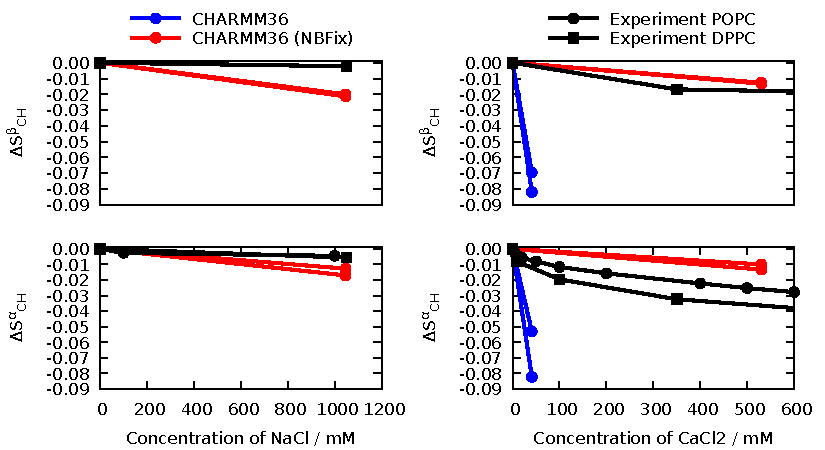
\includegraphics[width=17.0cm]{../Figs/OP_CHARMM_CaCl_POPC_NBFix.pdf}
  \caption{\label{OP_CHARMM_CaCl_POPC_NBFix}
    Headgroup order parameters from CHARMM36 simulations of POPC, where the NBfix term was employed employed for sodium \cite{venable13} ({\it left})
    and calcium \cite{kim16} ({\it right}) compared with the experimental data \cite{akutsu81,altenbach84}
    and simulations without NBfix for the calcium.
    Simulation files without ions are available at Ref. \citenum{nencineCHARMM36popcT310K},
    with the NBfix term in sodium at Ref.~\citenum{CHARMM36withCaClNBfix}, 
    with the NBfix term in calcium at Ref.~\citenum{CHARMM36withCaClNBfix} and
    without the NBfix in calcium at Ref.~\citenum{charmmPOPC450mMCaClfiles}.
  }
\end{figure}

\begin{figure}[]
  \centering
  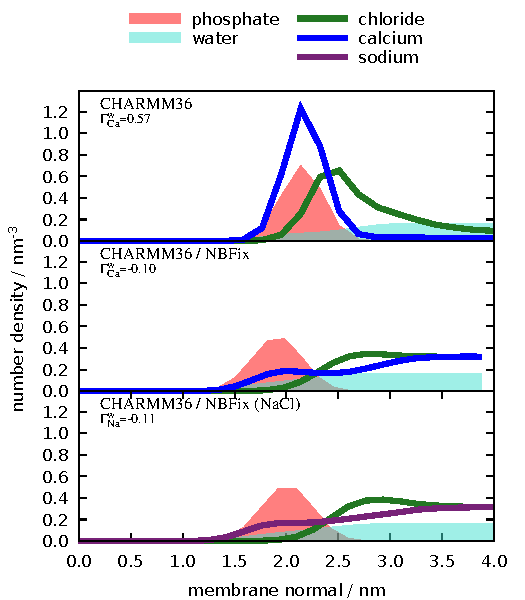
\includegraphics[width=17.0cm]{../Figs/density_profile_CHARMM_CaCl_POPC_NBFix.pdf}
  \caption{\label{density_profile_CHARMM_CaCl_POPC_NBFix}
    Density profiles along membrane normal from CHARMM36 simulations with (middle)
    and without (top) the NBfix term for calcium \cite{kim16} compared to the simulation
    with the NBfix term for sodium \cite{venable13} (bottom). The simulation data are the same as in Fig.~\ref{OP_CHARMM_CaCl_POPC_NBFix}.
  }
\end{figure}


\clearpage
\section{Calcium density profiles from simulations with \\ POPC:POPS(5:1) mixture}
%\todo{This section could benefit from some clarifying text}
\begin{figure}[ht]
  \centering
  \includegraphics[width=10cm]{../Figs/CAdensPCPSmixture.eps}
  \caption{\label{CAdensPCPSmixtureALL}
    Number density profiles of Ca$^{2+}$ from POPC:POPS (5:1) mixtures simulated with different force fields. The ion densities are taken along the z-axis that coincides with the bilayer normal. 
  }
%  \todo{Should we include also counterions into the plot?} \\
\end{figure}

\clearpage
\section{Details of the rough subjective force field ranking (Fig.~\ref{comparisonTablePS})} 

\section{Details of the force field ranking (Fig.~\ref{comparisonTablePS})}\label{Ranking} 
In Figure~\ref{HGorderParametersPS}) of main text we present a rough and subjective ranking of the force fields investigated in this work. 
The assessment was based on the data presented in Fig.~\ref{HGorderParametersPS}.
%
For each carbon (the columns in Fig.~\ref{HGorderParametersPS}),
we first investigated separately how well a given force field represents the {\bf magnitude} of the order parameters and their {\bf forking}.

\subsubsection*{Magnitude}
To quantify how close to the experimentally obtained C--H order parameters ($S_\mathrm{CH}$s) were to the 
the force-field-produced $S_\mathrm{CH}$s, we assign a number for each carbon based on the following 5-step scale:

%
\begin{description}
\item [0 (~):] \noindent {More than half of all the calculated $S_\mathrm{CH}$s (includes all hydrogens bound to that carbon and all lipid types investigated for the given force field) were within the {\it subjective sweet spots} (SSP, blue-shaded areas in Fig.~\ref{HGorderParametersPS}).}
%
\item [1 ({\textsf{\tiny M}}):] \noindent {All the calculated $S_\mathrm{CH}$s  were $< 0.03$ units away from the SSP.}
%
\item [2  ({\textsf{\small M}}):] \noindent {All the calculated $S_\mathrm{CH}$s  were $< 0.05$ units away from the SSP.}
%
\item [3 ({\textsf{\large M}}):] \noindent {All the calculated $S_\mathrm{CH}$s  were $< 0.10$ units away from the SSP.}
%
\item [4 ({\textsf{\Large M}}):] \noindent {Some of the calculated $S_\mathrm{CH}$s  were $> 0.10$ units  away from the SSP.}
\end{description}

\subsubsection*{Forking}
Forking in each force field was assessed based on how well the difference in order parameters of two hydrogens attached to a given carbon matched that obtained experimentally. Note that this is not relevant for $\beta$ and $\mathrm{g_2}$, which have only one hydrogen. For the $\alpha$ carbon,  for which a considerable forking of 0.105 is experimentally seen, the following 5-step scale was used:
\begin{description}
\item [0 (~):] \noindent {The distance $D$ between the symbols (indicating time-weighted averages in Fig.~\ref{HGorderParametersPS}) was $0.08 < D< 0.13$ units for all the calculated $S_\mathrm{CH}$s (includes all lipid types investigated for a given force field).}
%
\item [1 ({\textsf{\tiny F}}):] \noindent {$(0.06 < D < 0.08)$ OR $(0.13 < D < 0.15)$.}
%
\item [2  ({\textsf{\small F}}):] \noindent {$(0.04 < D < 0.06)$ OR $(0.15 < D < 0.17)$.}
%
\item [3 ({\textsf{\large F}}):] \noindent {$(0.02 < D < 0.04)$ OR $(0.17 < D < 0.19)$.}
%
\item [4 ({\textsf{\Large F}}):] \noindent {$(D<0.02)$ OR $(0.19<D)$.}
\end{description}
%
For the $\mathrm{g_3}$ carbon, for which no forking is indicated by experiments, the following 5-step scale was used:
%
\begin{description}
\item [0 (~):] \noindent {$ D< 0.02$.}
%
\item [1 ({\textsf{\tiny F}}):] \noindent {$0.02 < D < 0.04$.}
%
\item [2  ({\textsf{\small F}}):] \noindent {$0.04 < D < 0.06$.}
%
\item [3 ({\textsf{\large F}}):] \noindent {$0.06 < D < 0.08$.}
%
\item [4 ({\textsf{\Large F}}):] \noindent {$0.08 < D$.}
\end{description}
%
For the $\mathrm{g_1}$ carbon, for which a considerable forking of 0.13 is experimentally seen, the following 5-step scale was used:
%
\begin{description}
\item [0 (~):] \noindent {$0.11 < D < 0.15$.}
%
\item [1 ({\textsf{\tiny F}}):] \noindent {$(0.09 < D < 0.11)$ OR $(0.15 < D < 0.17)$.}
%
\item [2  ({\textsf{\small F}}):] \noindent {$(0.07 < D < 0.09)$ OR $(0.17 < D < 0.19)$.}
%
\item [3 ({\textsf{\large F}}):] \noindent {$(0.05 < D < 0.07)$ OR $(0.19 < D < 0.21)$.}
%
\item [4 ({\textsf{\Large F}}):] \noindent {$(D<0.05)$ OR $(0.21<D)$.}
\end{description}

\noindent Based on these assessments of magnitude and forking deviations from experimental values,
each carbon was then assigned to one of the following groups: "within experimental error"
(magnitude and forking deviations both on 0 of the scales described above),
"almost within experimental error"
(sum of the magnitude and forking deviation 1 or 2),
"clear deviation from experiments"
(sum of magnitude and forking deviation from 3 to 5), and
"major deviation from experiments"
(sum of magnitude and forking deviation from 6 to 8).
These groups are indicated by colors in Fig.~4.
(Note that for $\beta$ and $\mathrm{g_2}$, for which there can be no forking,
the corresponding group assignment limits were: 0, 1, 2, and 3.)

Finally, the total ability of the force field to describe the headgroup and
glycerol structure was estimated.
To this end, the groups were given the following weights:
0 (within experimental error),
1 (almost within experimental error),
2 (clear deviation from experiments),
4 (major deviation from experiments),
and the contributions from the five carbons were summed up.
The sum, given in the $\Sigma$-column of Fig.~\ref{HGorderParametersPS},
was then used to (roughly and subjectively) rank the force fields.

\section{Author contributions}
\noindent
{\it Hanne Antila}
contributed to the development of analysis tools used for evaluating the force fields,  provided critical discussion on the manuscript content, and edited it for clarity.

\noindent
{\it Pavel Buslaev}
analysed the dihedral angle distributions in the head group and glycerol backbone regions.

\noindent
{\it Fernando Favela-Rosales}
set up and performed one of the DOPS simulations with Slipids.

\noindent
{\it Tiago M. Ferreira}
performed the NMR experiments and NMR simulations, processed and analysed the experimental data, prepared the corresponding figures, wrote parts of the manuscript (NMR methods and interpretation of the SDROSS results), and took part in the final revision.

\noindent
{\it Ivan Gushchin}
supervised the work of P.B.

\noindent
{\it Matti Javanainen}
performed most of the MacRog simulations, and provided comments on the manuscript.

\noindent
{\it Batuhan Kav}
set up, performed, and analysed Amber Lipid14/17 simulations with the Amber MD.

\noindent
{\it Jesper J. Madsen}
set up, performed, and analysed several of the CHARMM36 simulations. Provided comments on the manuscript.

\noindent
{\it Josef Melcr}
consulted the project, 
prepared tools for calculating order parameters,
and performed several simulations.

\noindent
{\it Markus S. Miettinen}
worked with
H. A. on the analysis tools, and with
B. K. on the Amber MD simulations.
Made the subjective force field ranking.
Edited the manuscript.

\noindent
{\it Ricky Nencini}
ran the simulations of POPC systems using CHARMM36 with and without NB-Fix, and contributed to the discussion on system/bulk concentration. 


\noindent
{\it O. H. Samuli Ollila}
designed the project and managed the work.
Ran and analysed several simulations. Wrote the manuscript.

\noindent
{\it Thomas J. Piggot}
set up, performed, and analysed many of the simulations. Contributed to parts of the manuscript.

\clearpage
\bibliography{refs.bib}

\end{document}
